%%%%%%%%%%%%%%%%%%%%%%%%%%%%%%%%%%%%%%%%%%%%%%%%%%%%%%%%%%%%%%%%%%%%%%%%%%%%%%%%%%%%%%%%%%%%%%%%%%%%%
% This template is distributed with ABSOLUTELY NO WARRANTY.
% It serves as a guideline and constitutes a basic structure for a
% thesis/dissertation. The user assumes full responsibility for formatting
% and typesetting their document and for verifying that all the thesis
% requirements set by the University of Tennessee are met. Please refer to the most
% recent UT thesis guide (http://web.utk.edu/~thesis/thesisresources.shtml)
% or contact the thesis consultant (http://web.utk.edu/~thesis/).
% Please report any bugs to the thesis consultant.
%%%%%%%%%%%%%%%%%%%%%%%%%%%%%%%%%%%%%%%%%%%%%%%%%%%%%%%%%%%%%%%%%%%%%%%%%%%%%%%%%%%%%%%%%%%%%%%%%%%%%
% O P T I O N S:
% 1. thesis/dissertation
% 2. monochrome
% 3. all options provided by the report class
%\documentclass[thesis,letterpaper,12pt]{utthesis} % thesis, one side
% some alternatives are:
%\documentclass[thesis,monochrome,letterpaper,12pt]{utthesis} %thesis, one side, monochrome text
%\documentclass[thesis,twoside,letterpaper,12pt]{utthesis} % thesis, two side
%\documentclass[thesis,monochrome,twoside,letterpaper,12pt]{utthesis} % thesis, two side, monochrome text
% for a dissertation, replace the thesis option by dissertation:
\documentclass[dissertation,letterpaper,12pt]{utthesis}
\renewcommand{\baselinestretch}{1.5} 	 % line Spacing
%%%%%%%%%%%%%%%%%%%%%%%%%%%%%%%%%%%%%%%%%%%%%%%%%%%%%%%%%%%%%%%%%%%%%%%%%%%%%%%%%%%%%%%%%%%%%%%%%%%%%
% TO DO: FILL IN YOUR INFORMATION BELOW - READ THIS SECTION CAREFULLY
%%%%%%%%%%%%%%%%%%%%%%%%%%%%%%%%%%%%%%%%%%%%%%%%%%%%%%%%%%%%%%%%%%%%%%%%%%%%%%%%%%%%%%%%%%%%%%%%%%%%%
\title{The EMC Effect in A=3 Nuclei}	       % title of thesis/dissertation
\author{Jason Earl Bane}                % author's name
\copyrightYear{2019}            % copyright year of your thesis/dissertation
\graduationMonth{December}           % month of graduation of your thesis/dissertation
%\majorProfessor{Nadia Fomin}	    % advisor's name
%\keywords{EMC, Nuclear Structure, Electron scatterning}	% keywords (optional) separated by commas - these are used in the PDF file properties
%\viceProvost{Carolyn R. Hodges} % vice provost name
%\major{Nuclear Physics}	% major: Mechanical Engineering, Aerospace Engineering, Mathematics...
\degree{Doctor of Philosophy}	    % degree: Doctor of Philosophy, Master of Science, Master of Engineering...
%\college{Arts and Sciences}           % college
%\dept{Physics and Astronomy}	% department
\university{The University  of Tennessee, Knoxville}	% school name
% THIS TEMPLATE ACCOMMODATES UP TO 5 COMMITTEE MEMBERS - ENTER ONLY THE NAMES OF THE MEMBERS ON YOUR COMMITTEE
%\numberOfCommitteeMembers{4} % enter the number of committee members
%\committeeMemberA {Jamie Coble}	% name of first committee member
%\committeeMemberB {Kate Jones}	% name of second committee member
%\committeeMemberC {Thomas Papenbrock}	% ... you get the trend!
%\committeeMemberD {Soren Sorensen}	% if your committee has less than 4 members, you do not need to edit the
%\committeeMemberE {Committee Member 5}  % rest of committee names
%%%%%%%%%%%%%%%%%%%%%%%%%%%%%%%%%%%%%%%%%%%%%%%%%%%%%%%%%%%%%%%%%%%%%%%%%%%%%%%%%%%%%%%%%%%%%%%%%%%%%
% LOAD SOME USEFUL PACKAGES
%%%%%%%%%%%%%%%%%%%%%%%%%%%%%%%%%%%%%%%%%%%%%%%%%%%%%%%%%%%%%%%%%%%%%%%%%%%%%%%%%%%%%%%%%%%%%%%%%%%%%
\usepackage{enumitem}
\usepackage{nomencl}                    % produces a nomenclature
\usepackage{float}                      % figure floats
\usepackage{natbib}                     % this package allows you to link your references
\usepackage{graphicx}					% graphics package
\graphicspath {{images/}} % specify the path where figures are located
\usepackage{fancyhdr}                   % fancy headers and footers
\usepackage{url}                      % nicely format url breaks
\usepackage[inactive]{srcltx}		 	% necessary to use forward and inverse searching in DVI
\usepackage{relsize}                    % font sizing hierarchy
\usepackage{booktabs}                   % professional looking tables
\usepackage[config, labelfont={bf}]{caption,subfig} % nice sub figures
\usepackage{tikz}
\usepackage{multicol}
\usepackage{rotating}
\usepackage{pdflscape}
%\usepackage{floatrow}
\usepackage[outdir=./images/]{epstopdf}
%%/lin\usepackage{csvsimple}
\usepackage{relsize}                    % font sizing hierarchy
\usepackage[titletoc]{appendix}			% format appendix correctly
\usepackage[absolute]{textpos}
\usepackage{fancyhdr}
\usepackage[titletoc]{appendix}			% format appendix correctly
\usepackage{lineno}
%\linenumbers
\usepackage{mathrsfs}                   % additional math scripts
%%% PACKAGES THAT ARE PRELOADED WITH THE CLASS ARE: amsmath,amsthm,amssymb,setspace,geometry,hyperref,and color
\usepackage{chngcntr}
\usepackage{lscape}

\fancypagestyle{lscape}{% 
	\fancyhf{} % clear all header and footer fields 
	\fancyfoot[CE]{%
		\begin{textblock}{20}(1,5){\rotatebox{90}{\leftmark}}\end{textblock}
		\begin{textblock}{1}(13,10.5){\rotatebox{90}{\thepage}}\end{textblock}}
	\fancyfoot[CO] {%
		\begin{textblock}{1}(13,8){\rotatebox{90}{\thepage}}\end{textblock}
		\begin{textblock}{20}(1,13.25){\rotatebox{90}{\rightmark}}\end{textblock}}
	\renewcommand{\headrulewidth}{0pt} 
	\renewcommand{\footrulewidth}{0pt}}




%%%%%%%%%%%%%%%%%%%%%%%%%%%%%%%%%%%%%%%%%%%%%%%%%%%%%%%%%%%%%%%%%%%%%%%%%%%%%%%%%%%%%%%%%%%%%%%%%%%%%
\begin{document}
	\renewcommand{\topfraction}{0.45}
	\renewcommand{\textfraction}{0.5}
	\setlength{\textfloatsep}{0.45in} 
    \pagenumbering{alph} % this is needed to clear certain issues with the hyperref package
%
\addToPDFBookmarks{0}{Front Matter}{rootNode} % create a root node named "Front Matter" in the pdf bookmarks
\addToPDFBookmarks{1}{Title}{a} % add a pdf bookmark to the title page
\makeTitlePage % make the title page.
%
\pagenumbering{roman}
\setcounter{page}{2}
%
\makeCopyrightPage % make the copyright page
%
%%%%%%%%%%%%%%%%%%%%%%%%%%%%%%%%%%%%%%%%%%%%%%%%%%%%%%%%%%%%%%%%%%%%%%%%%%%%%%%%%%%%%%%%%%%%%%%%%%%%%
%The dedication and acknowledgments are optional. If you wish not to include them, simply comment out both the "\addToPDF..." line and the "\include{...}" line for each.
%%%%%%%%%%%%%%%%%%%%%%%%%%%%%%%%%%%%%%%%%%%%%%%%%%%%%%%%%%%%%%%%%%%%%%%%%%%%%%%%%%%%%%%%%%%%%%%%%%%%%
\addToPDFBookmarks{1}{Dedication}{b} % add a pdf bookmark to the dedication page
\include{front-matter/dedication} % include the dedication

\addToPDFBookmarks{1}{Acknowledgments}{c} % add a pdf bookmark to the acknowledgments page
\begin{center}
	{\large \textbf{Acknowledgments}}\\
\end{center}

\paragraph{}I would like to thank everybody that played a role in completing this step of my life. I know there is no way that I could go one by one through every person that helped and thank them. I am sure that it would take too many pages and then I would leave somebody out. There are a few special people, that I would like to call out. 
\paragraph{}First, I would like to thank my brother, James for the courage to change career paths and my parents, Barb, Howard, and Deb for the support and guidance. Thanks to Dallas and Jennifer, for housing me for a few months. Thank you Dr. Fomin for targeting my weakness, the beach, and giving me the chance to join the JLab community. Also, I would like to thank Dr. Fomin for supporting my research and guiding me though the swamps of PhD. research. I would like to thank the JLab community specially Dr. Higinbotham for accepting me into the community and helping through this journey including keeping the office door open for me to drop in a million times! I would also like to thank my committee for guiding me through my defense and allowing me to graduate. 
\paragraph{}I would really like to thank the extended tritium family of grad students and post docs. Working with such a great group of people from around the world has truly been amazing!! Thank you, Sheren, Scott, Jessica, Tyler H., Hanjie, Dien, Mike, Tong, Shujie, Rey, Johnathan, Tyler K., Nathaly, Bishnu, Evan, Florian, Luke, Marco, and Zhihong. Lastly and I think the person deserving of the most thanks, is my wife, Callie. Thank you so much for everything! Specially thank you for dropping everything and coming on this adventure with me!.

\paragraph{}I would like to thank the DOE and JSA for financial support throughout my time at JLab.  % include the acknowledgments

\addToPDFBookmarks{1}{Abstract}{e} % add a pdf bookmark to the abstract page
\begin{center}
	{\large \textbf{Abstract}}\\
	
	{\large \textbf{The EMC Effect in A=3 Nuclei}}\\
\end{center}

The European Muon Collaboration(EMC) discovered an unexpected and puzzling result in 1983 when comparing the deep inelastic scattering(DIS) nuclear structure functions of Deuterium and Iron. The per-nucleon structure functions were found to be different for the two nuclei, rather than a simple average over the proton and neutron structure functions.  In subsequent experiments, this phenomenon was confirmed for additional nuclei, with the magnitude approximately scaling with the density.  The exact mechanism leading to this in-medium structure function modification has not been identified.  I will discuss recent results from JLab exploring the EMC effect by using an electron beam to probe two mirror nuclei, Helium-3 and Tritium. 
 % your abstract

\addToPDFBookmarks{0}{Table of Contents}{f}
\tableofcontents % generate a table of contents
\listoftables % generate a list of tables
\listoffigures % generate a list of figures

\newpage
\pagenumbering{arabic}
\setcounter{page}{1}
%%%%%%%%%%%%%%%%%%%%%%%%%%%%%%%%%%%%%%%%%%%%%%%%%%%%%%%%%%%%%%%%%%%%%%%%%%%%%%%%%%%%%%%%%%%%%%%%%%%%%
% INCLUDE THE CHAPTERS STARTING WITH THE NOMENCLATURE IF PRESENT
%%%%%%%%%%%%%%%%%%%%%%%%%%%%%%%%%%%%%%%%%%%%%%%%%%%%%%%%%%%%%%%%%%%%%%%%%%%%%%%%%%%%%%%%%%%%%%%%%%%%%
						
     	


\chapter{Introduction}\paragraph{}Understanding the world around us is the goal of every scientist, from the chemist that experiments with the formation of atoms to the geologist exploring the process of rock formations. Nuclear physicists focus on studying the fundamental constituents of matter, the building blocks of nature. Physicist use scattering experiments at accelerator facilities, like CERN in Switzerland, DESY in Germany, BATES in Massachusetts, JLab in Virginia, and many others, to study the protons and neutrons that make up a nucleus and the constituents that make up the internal structure of a nucleon. These experiments allow physicists to probe inside a nucleus to observe the internal structure and to investigate the interactions between the quarks and gluons. Many of the experiments are design to confirm an existing results while also expanding on unique ideas.
\paragraph{}In the last century, there have been numerous breakthroughs in the fields of nuclear and particle physics. Rutherford discovered the proton by bombarding light nuclei with alpha particles to produce the reaction,  
	\begin{equation}
	^{14}N + ^4He \rightarrow ^{17}O + p.
	\end{equation}
This reaction allowed Rutherford to conclude that the Hydrogen nucleus was a elementary constituent of atomic nuclei \cite{PnN}. In the late 1950s, experimental results published by W. McAllister and R. Hofstadter exposed some of the eternal structure of the proton \cite{Flay,Hof}. The European Muon Collaboration(EMC) produced results in the early 1980s showing a difference between the internal structure of the deuterium nucleus and Iron \cite{seeley,CC}. In the current era, scientific labs can produce beams of leptons, hadrons, and heavy ions. These beams can be produced with a large energy spread from "cold" neutrons of $10^{-2}eV$ to protons of $10^{12}eV$. The data received from scattering experiments using beams with a complex structure like alpha particles of heavy ions contain information about the target, the beam, and the interaction between the two. 
\paragraph{}This thesis will discuss using deep inelastic scattering to study the internal structure of two light nuclei and gain a better understanding of the effects of the slight difference between these two light nuclei as part of the E12-010-103 experiment. The discussion will include the motivations, approach, and the outcome from one analysis technique.

\section{Electron scattering}\label{sec:escat}
\paragraph{}Deciphering and analyzing data from scattering experiments that use complex beams can be convoluted because the scattering interaction contains information about the internal structure of the target and the beam along with the complex interactions and forces between the two \cite{PnN}.  In order to remove some of the complexity in scattering experiments, one may employ highly relativistic electrons. Electrons being point-like particles without any internal structure allow the elimination of some of the analysis difficulties due to the complex nature of the internal structure of more complex scattering tools. Electrons and the target either a nucleus, nucleon, or quark interact via the exchange of a virtual photon. Using quantum electrodynamics (QED), these interactions can accurately be described by the well known electromagnetic interaction.
\paragraph{}The electromagnetic interaction describes the coupling of fundamental particles via their electric charge. The interaction between two electrically charged particles begins when a virtual photon is emitted. The amplitude for the emission of photon is proportional to $\sqrt{\alpha}$. Where $\alpha$ is the fine structure constant. Higher order terms of this process contribute very little due to the coupling constant $\alpha \approx 1/137 $, being much smaller than one. 
\paragraph{} The Feynman diagram in figure \ref{feynman} represents an electron scattering from a proton. The incoming or incident electron's four-momentum is described as k = (E,$ \vec{k}$) and the scattering electron's four-momentum is represented by $k^\prime{}$ = ($E^\prime{}$,$\vec{k}^\prime{}$). The exchange of the virtual photon in this electromagnetic interaction is defined by the four-momentum transfer q. $Q^2$, the square of the momentum transfer is the mass of the virtual photon that interacts with the hadron. 
\begin{equation}
\label{Q}
Q^2 \equiv -q^2 = 4EE^\prime{} sin^2(\theta/2).
\end{equation} 
In equation \ref{Q}, E is the electrons incident energy and E$^\prime$ is the energy of the scattered electron. Theta is the angle that describes the deflection of E$^\prime$ vector from the electron's incident path. 
\begin{figure}[h]
\centering
\caption{Simple Feynman diagram of an electron scattering from a proton \cite{Flay}.}
\includegraphics[width=10cm]{feyman_e_p.png}
\label{feynman}
\end{figure}
Along with $Q^2$, the variables $\nu$, W, and $x_B$  are used to narrate the evolution of the electron scattering process. $\nu$, defined as $P\cdot q/M$. Where $P$ is the 4-vector of the target proton. In the laboratory frame, $\nu$ can be described by \ref{v}. The transformation to laboratory frame allows the use of the resting nature of the target proton. Therefor $P = (Mc,\boldsymbol{0})$ and $ q = (( E-E\prime)/c,\boldsymbol{q})$. 
\begin{equation}
\label{v}
\nu = E - E^\prime{}.
\end{equation}
Simply, $\nu$ is the magnitude of energy loss by the electron during the scattering interaction. The invariant mass of the system, W,  defines the hadronic state produced by the scattering event. 
\begin{equation}
\label{W}
W^2 \equiv (q + p)^2 = M^2 + 2M\nu -Q^2.
\end{equation}
In the general case of electron scattering off of a free proton or neutron elastically, the scattered energy of the electron will be a function of the incident electron's energy and the scatted angle of the electron, shown in the following equation.
\begin{equation}
E^\prime =\frac{E}{1+\frac{E}{Mc^2}(1-cos\theta)}
\end{equation}
A scattering event with the invariant mass equal to the the mass of the nucleon, $M$, falls in the regime of elastic scattering and the final state of hadron is a recoiling proton. Increasing the $W$ above $M$ will transform the scattering interaction from an elastic scattering interaction to an inelastic scattering event due to the excited state of the scattered byproduct. 
\paragraph{} The intrinsic likelihood of an event with a certain $Q^2$, $\nu$, and $W$ is defined by the scattering cross section. An electron scattering off of a target with a charge of $Z*e$ can be described by the Rutherford cross-section. Povh et. al. details the Rutherford cross section as:
\begin{equation}
\bigg(\frac{d\sigma}{d\Omega}\bigg)_{Rutherford} = \frac{ \big(zZe^2\big)^2} {\big( 4\pi \epsilon_0\big)^2 * \big(e E_{kin}\big)^2 sin^4\big( \theta / 2 \big) }. 
\end{equation}
In the early 1920s, German physicists Stern and Gerlach performed an experiment with a beam of silver atoms. The Stern–Gerlach experiment measured the deflection of a beam of silver atoms from an inhomogeneous magnetic field\cite{strger}. The observations made by Stern and Gerlach demonstrated that particles bear an intrinsic angular momentum. In 1925, a forbidden spectral line of ionized helium raised questions of the current understanding of the quantum numbers used. This forbidden line lead to the discovery of electron spin by Uhlenbeck and Gloudsmit\cite{e_spin}. The Mott cross-section is the evolved version of the Rutherford cross-section. The Rutherford cross-section neglects the spin of an electron and the target. Evolving the Rutherford cross-section allows for the modifications needed to include the intrinsic spin of the target and electron. The Mott cross-section is described in equation \ref{Mott} \cite{HighE,PnN}.  Where $\alpha$ is the fine structure constant. This constant is related to the strength of the interaction between an electron and proton\cite{sane}.
\begin{equation}
\bigg(\frac{d\sigma}{d\Omega}\bigg)_{Mott} = \frac{4Z^2\alpha^2 \big(\hbar c \big)^2 E{^{\prime} }^2}{ |\boldsymbol{q}c|^4} cos^2 (\theta/2). \label{Mott}
\end{equation}
The inclusion of the interaction between the current of the electron and the target nucleon's magnetic moment creates the necessity to define the magnetic moment. Equation \ref{magmom} describes the magnetic moment of a charged, spin -1/2 particle. The magnetic momentum is build using M, the mass of the particle and g, a factor of 2 relating to relativistic quantum mechanics. 
\begin{equation}
\mu = g \cdot \frac{e}{2M}\cdot\frac{\hbar}{2} \label{magmom}
\end{equation}
Modifying the Mott scattering cross section equation to include a spin degree of freedom, is shown in equation \ref{spin.5}. $\tau$ is used in the cross section formalism to account for the magnetic moment of a nucleon and is defined as: $\tau = \frac{Q^2}{4M^2c^2}$ \cite{PnN}. 
\begin{equation}
\bigg(\frac{d\sigma}{d\Omega}\bigg)_{\substack{point \\ spin 1/2}} = \bigg(\frac{d\sigma}{d\Omega}\bigg)_{Mott} \cdot \big[1 + 2\tau \: \text{tan}^2\frac{\theta}{2} \big]\label{spin.5}
\end{equation}

\begin{figure}[]
	\centering
	\textbf{ }\par\medskip
	\includegraphics[width=10cm]{mott_exp.pdf}
	\caption{Ratio of experimentally measured cross section to the Mott  cross-section verses tan$^2\theta/2$ for a $Q^2$ of 2.5 GeV$^2$/c$^2$. \cite{EPinter}}
	\label{mott_exp}
\end{figure}

\paragraph{}The interaction described in the Mott cross section equation is mediated by a single photon and is electromagnetic in nature. For an electromagnetic interaction conducted at a low resolution, there is an agreement between the measured cross section and the theoretical Mott cross-section. This agreement is maximized when in the limit of $|\boldsymbol{q}| \rightarrow  0$ for scattering events of electrons off of a target nuclei. As $|\boldsymbol{q}|$ climbs furtherer from zero and the resolution of probe grows, the experimentally measured cross sections will begin to differ from the Mott cross section, systematically decreasing \cite{PnN}. The comparison of the Mott calculated cross section to experimentally measured cross section for a $Q^2$ of 2.5 GeV$^2$/c$^2$ is shown in figure \ref{mott_exp}. Increasing the $|\boldsymbol{q}|$ of an interaction reduces the size of the wavelength of the virtual photon that mediates the electromagnetic interaction between the electron and target nuclei and therefor increases the resolution of the probe. The wavelength of this virtual photon is inversely proportional to $|\boldsymbol{q}|$, and can be described by the following: $\lambda = \ \frac{\hbar}{|\boldsymbol{q}|}$ \cite{PnN}. Increasing the amount of momentum transfered in an electromagnetic reaction allows one to study deeper into the nucleus. The act of probing deeper into the nucleous or nucleon allows for the substructure of the target. 
\paragraph{} Studying the internal structure of a nucleus with the electromagnetic interaction requires increasing the momentum transfered. Pushing $|\boldsymbol{q}|$ to be comparable with the mass of a nucleon adds more complexity to the details of the scattering interaction. At the appropriate levels of $|\boldsymbol{q}|$ to study the nucleons in the nucleus, the Mott cross-section equation requires modifications to include additional factors that incorporate information about the target. The Rosenbluth formula is based on the Mott cross section and embraces target recoil, magnetic moment, and charge and current distributions. Povh writes the Rosenbluth formula as:
\begin{equation}
\label{rosen}
\bigg(\frac{d\sigma}{d\Omega}\bigg)=\bigg(\frac{d\sigma}{d\Omega}\bigg)_{Mott} *\bigg\lbrack \frac{G^2_E(Q^2) +\tau G^2_M(Q^2)}{1+\tau} + 2\tau G^2_M(Q^2)tan^2\frac{\theta}{2} \bigg\rbrack.
\end{equation}
Equation \ref{rosen} contains $G^2_E(Q^2)$ and $G^2_M(Q^2)$, the electric and magnetic form factors. These form factors depend on $Q^2$, and this measured dependence provides information on the radial charge distributions and magnetic moments of the scattering participants. 

\begin{align}
	\begin{split}
		&G^P_E(Q^2=0) = 1 \\
		&G^P_M(Q^2=0) = 2.79
	\end{split}
	\begin{split}
	    &G^n_E(Q^2=0) = 0 \\
	    &G^n_M(Q^2=0) = -1.91 \label{FFeq}
	\end{split}
\end{align}



\subsection{Deep inelastic scattering}\label{sec:DIS}
\paragraph{}The first generation of electron scattering experiments achieving a significantly large  $|\boldsymbol{q}|$ used a linear accelerator with a 25 GeV maximum beam energy, and following generations increased the total interaction energy to substantially higher thresholds. At these high incident beam energies, individual resonances cannot be separated in the invariant mass spectrum above 2.5 GeV. Observations made into this convoluted invariant mass spectrum has shown that many strongly interacting particles are produced, known as hadrons. Scattering interactions that generate these hadrons are considered to be inelastic. 
\paragraph{}Inelastic scattering events contain the possibility of conceiving additional resultants causing an increase in the complexity of a scattering interaction. In order to create an inelastic event, the wavelength of the virtual photon has to be comparable to the radius of the struck nucleon. Increasing the amount of transferred momentum so that $Q^2R^2 \gtrsim 1$, will increase the resolution of the probe to a level that allows for the interaction to be with the charge constituents within the nucleon. When the scattering event probes the fundamental elements of a nucleon, the scattering process is titled deep inelastic scattering(DIS). Due to the increase in complexity, an additional degree of freedom has to be introduced into the scattering cross section formalism. Modifying the Rosenbluth formula to include the inelastic scattering structure functions $F_1(Q^2,\nu)$ and $F_2(Q^2,\nu)$ evolves the Rosenbluth formula to contain the needed complexity of an inelastic event. These modifications are shown in equation \ref{ISCS}. The $F_1$ and $F_2$ structure functions provide the details for describing the internal composition of the nucleon \cite{PnN}. 




\begin{equation}
\label{ISCS}
\frac{d^2\sigma}{d\Omega dE^\prime}=\bigg(\frac{d\sigma}{d\Omega}\bigg)_{Mott} \bigg\lbrack \frac{F_2(Q^2,\nu)}{\nu} + \frac{2F_1(Q^2,\nu)}{M}tan^2\frac{\theta}{2} \bigg \rbrack.
\end{equation}  
\paragraph{}In the case of DIS off of a proton, the electron probe is used to explore the exclusive internal structure of the proton. In 1969, Feynman assumed the internal make up of the proton was that of point-like partons \cite{Briskin_thesis,DISproton}, the basis of the parton model. As part of this model, the impulse approximation makes an assumption that the duration of the interaction between the mediating photon and parton is relatively short, allowing for the interaction between individual partons to be neglected. Thus in a DIS interaction, the partons can be described as free, with minimal internal interactions. Under this understanding, a electron-nucleon DIS interaction would characterize the properties and motions of the partons that make up the struck nucleon\cite{DISproton}. The characteristics, the motions and properties, of the partons are formalized into a parton distribution function $f_i(x_B)$. The Bjorken scaling variable, $x_B$ or $x$, is a dimensionless quantity that measures the in-elasticity of a scattering process and is defined as: $x \equiv \frac{Q^2}{2M\nu}$. The parton distribution functions can be used to relate the $F_1$ and $F_2$ structure functions used in equation \ref{ISCS} \cite{PnN}. 
\begin{align}
	\label{PDFs}
	F_2(x) &= x \Sigma_i e^2_i f_i(x)\\
	F_1(x) &= \frac{1}{2x} F_2(x) \nonumber
\end{align}
\begin{equation}
\label{F2q}
F_2(x) = x1 \cdot \Sigma_f z^2_f ( q_f(x) + \bar{q}_f(x))
\end{equation}

\paragraph{} Measurements from the Standford Linear Accelerator(SLAC) 
 In the Bjorken limit, v $\rightarrow \infty$ and $Q^2 \rightarrow \infty$, the deep inelastic structure functions can be described as functions of only $x$.

\begin{figure}[H]
	%	\hspace*{-20pt}
	\centering
	\includegraphics[width=10cm]{SLAC_F2.png} 
	\caption{ Measurement of the proton structure function $F_2(x, Q^2)$\cite{ref:rev_pp} .}
	\label{F2_fig}
\end{figure} 


\begin{figure}[]
	\centering
	\includegraphics[width=7.5cm]{quarks.png} 
	\caption{ Table of leptons, quarks, and bosons with mass, charge and spin \cite{sane}.}
	\label{fig:quarks}
\end{figure} 

	\cite{DISearly}
	\cite{DISproton}
	\cite{whitlow_sigma}
	\cite{Q2indy}
	
	
	
\section{EMC Effect}\label{sec:EMC}
\paragraph{}The European Muon Collaboration (EMC) performed a deep inelastic measurement with 120-280 GeV muons on iron and deuteron targets \cite{challenge}. The EMC extracted A/D structure function ratios versus the Bjorken scaling variable, $x$.  The relationship originally expected by the EMC contained the sum of the structure functions of each nucleon in a nucleus. Each nucleus has a certain number of neutrons (N) and a amount of protons (Z). The expected structure function for a nucleus could be written as:
\begin{equation}
F_A = N F_2^N + ZF_2^P.
\end{equation}
 The EMC compared the extracted structure functions from iron and deuterium. Their results are shown in Figure \ref{EMCOld}. The $\frac{A}{D}$ structure function ratio showed an unexpected downward slope. This phenomenon was titled the EMC effect. This finding demonstrated to the EMC that their understanding of the nucleus was incorrect. A nucleon's structure function and thereby, the constituent quark distributions may be altered by the nucleus. 
\begin{figure}[h]
\centering
 \caption{ Graph of the ratio of A/D structure functions vs $x$ for Carbon \cite{CC}.}
 \label{EMCOld}
 \includegraphics[width=10cm]{EMC.png} 
 \end{figure} 

\paragraph{}Ever since the European Muon Collaboration discovered the depletion of quarks at high $x$ for A $>$2 nuclei, physicists have tried to discover its cause. Scientists at SLAC extracted structure function ratios for many nuclei including; $^4$He, $^9$Be, $^{12}$C, $^{27}$Al, $^{40}$Ca, $^{56}$Fe, $^{108}$Ag, and $^{197}$Au. There were slightly different results for each nucleus. The magnitude of the EMC effect, taken to be the A/D ratio at $x=0.6$, was found to be different for the various nuclei, and roughly scaled with the size or density of the nuclei. The NMC (New Muon collaboration), another group at CERN, gathered precise data in order to construct the inclusive cross section of deuterium and protons. BCDMS collaboration extracted data for N and Fe structure function ratios. Figure \ref{EMC3} shows some of the data from SLAC and BCDMS on the EMC effect for Iron and Cu. Figure \ref{EMC 1} shows this result from a recent JLab EMC measurement, most precise to date. Many models over the years have been able to reproduce the shape of the A/D ratios. These models can contain traditional nuclear physics effects like momentum distribution or pion-charge contributions. Some models also describe the EMC effect through quark momentum distribution or modification of the internal structure \cite{Norton, piler, arri, DF, gomez}. However, no single model has provided a complete picture of the possible underlying physics. Precise data from Jlab's E03-103 experiment has revitalized this research. This experiment focused on precision measurements in light nuclei and added $^{3}$He as a target nucleus. Instead of taking the A/D ratio at a certain $x$-value to be the magnitude of the EMC effect, this analysis looked at the slope instead. This eliminated sensitivity to normalization uncertainties.

\begin{figure}[h]
\centering
\caption{EMC effect from EMC, SLAC, and BCDMS \cite{Norton}}
\label{EMC3}
\centering
\includegraphics[width=10cm]{EMC3.png}
\end{figure}

\begin{figure}[h]
\centering
 \caption{ Graph of the ratio of A/D structure functions vs $x$ for Carbon \cite{CC}.}
 \label{EMC 1}
 \includegraphics[width=10cm]{EMC1.png} 
 \end{figure} 
 

\paragraph{} In Figure , $^9$Be was found not to follow the previously observed scaling with nuclear density. This result from Jefferson Lab determined that the previous idea of a dependence on A or nuclear density in the EMC effect to be incorrect \cite{seeley}. This result spawned a drive to determine another explanation for the EMC effect and understand what clue the $^9$Be outlier was providing. The structure of this nucleus is made up of two high-density alpha particles and a single neutron \cite{ajppt}. The regions of higher density that are contained in a comparatively large volume may be able to explain why $^9$Be does not follow the expected trend. This suggests that the EMC effect could be a function of local nuclear density \cite{seeley}. 




\section{MARATHON}
Experiment E12-010-102, MARATHON (MeAsurement of the $F2^n$/$F_2^p$,$d$/$u$ RAtios and A=3 EMC Effect in Deep Inelastic Electron Scattering Off the Tritium and Helium MirrOr Nuclei), will use deep inelastic scattering off of the mirror nuclei $^3$H and $^3$He to measure the EMC effect for both $^3$H and $^3$He, to determine the ratio of the neutron to proton inelastic structure functions, and to find the ratio of the down to up quark distributions in the nucleon.


    	\chapter{EMC Effect}	
\section{European Muon Collaboration}\label{sec:EMC}
\paragraph{}The European Muon Collaboration (EMC) performed a deep inelastic measurement with 120-280 GeV muons on iron, hydrogen, and deuteron targets to begin a comprehensive study of ,muon scattering \cite{challenge, Norton}. The EMC used muons in order to reach their goal of achieving interactions at a large $Q^2$ \cite{seelyth}. The EMC studied the per nucleon normalized Fe/D structure function ratio versus the Bjorken scaling variable, $x$. The EMC expectations for this ratio originally was unity for $x$ between 0.05 and 0.7 and would deviate at higher $x$ due to Fermi smearing\cite{CC}. The reasoning for this expectation was the belief that at large magnitude of $Q^2$ the interaction between protons and neutrons would not contribute to the total structure function of the nucleus. This was the understanding because the binding energy of a few MeV would not interferer with the GeV scale of the DIS interaction \cite{Ajth}. The expected structure function for a nucleus could be written as:
\begin{equation}
F_2^A = N F_2^N + ZF_2^P.
\end{equation}
In this quasi-free nucleon picture, the nucleons are used to build up the nuclear structure ($F_2^A$) by summing up the neutron structure function ($F_2^N$) with the proton structure function($F_2^P$) for each nucleon. Their results for their ration comparison of iron and deuterium are shown in Figure \ref{EMCOld}. The $\frac{A}{D}$ structure function ratio showed an unexpected downward slope. This phenomenon was titled the EMC effect. This finding demonstrated to the EMC that their understanding of the nucleus was incorrect. A nucleon's structure function and thereby, the constituent quark distributions are altered by the structure of the nuclear medium. 
\begin{figure}[h]
	\centering
	\caption{ Graph of the ratio of A/D structure functions vs $x$ from the EMC. \cite{CC,EM}.}
	\label{EMCOld}
	\includegraphics[width=10cm]{EMC.png} 
\end{figure} 
\section{Ratios - Cross Sections and Structure Functions}
\paragraph{}In chapter one we defined the  inelastic cross section in equation \ref{ISCS}.  
\begin{equation}
\label{ISCSch2}
\sigma^A=\frac{4\alpha^2E^{\prime 2}}{Q^4} \bigg\lbrack 2\frac{F_1^A(x)}{M}sin^2\frac{\theta}{2} + \frac{F_2^A(x)}{\nu}cos^2\frac{\theta}{2} \bigg \rbrack.
\end{equation} 
In figure \ref{EMCOld}, the EMC collaboration analyze the ratio of $F_2$ structure functions. The per nucleon cross section of two different nuclei can be reduced to ratio of the $F_2$ structure functions.  
\begin{equation}
\label{rat}
\frac{\sigma_{A_2}}{\sigma_{A_1}} = \frac{F_2^{A_2}}{F_2^{A_1}}
\end{equation}
The reduction of the ratio of two nuclei begin by using the ratio of longitudinal and transverse cross sections as a function of $F_1/F_2$.
\begin{equation}
R=\frac{\sigma_{L}}{\sigma_{T}} =\left(1+\frac{\nu^2}{Q^2} \right)\frac{MF_2}{\nu F_1} -1
\label{Rratio}
\end{equation}
The ratio of two unique per nucleon cross sections is:
\begin{equation}
\label{Aratio}
\frac{\sigma_{A_2}}{\sigma_{A_1}} = \frac{F_2^{A_2}}{F_2^{A_1}} \frac{\left[1+ 2\frac{\nu F_1^{A_2} }{MF_2^{A_2}} tan^2\frac{\theta}{2} \right]}{\left[1+ 2\frac{\nu F_1^{A_1} }{MF_2^{A_1}} tan^2\frac{\theta}{2} \right]}
\end{equation}
Where $A_1$ and $A_2$ denote the different nuclei. Using the definition of $R$ in equation \ref{Aratio}, the per nucleon cross section ratio of $A_1$ and $A_2$ can be simplified to equation \ref{rat} \cite{EM,seelyth}. The simplification of the cross section ratio to the structure function ratio is based on the use of $R$. The longitudinal and transverse cross section ratio has been study extensively for many nuclei. The measurements of $R$ have shown no dependence on the number of nucleons \cite{EM}. 
\paragraph{}The $x$ spectrum of a per nucleon cross section ratio of some nucleus with A nucleons and deuterium also known as an $A/D$ ratio or an EMC ratio is broke into 4 different regions. 
\begin{itemize}
	\item For $x < 0.1$, the shadowing region has an EMC ratio that shows a decline of the nuclear stricture functions. A coupling of the photon to strongly interacting quarks causes this feature \cite{PnN}.
	\item The anti-shadowing region of the $x$ spectrum lies at $0.1 \leq x < 0.3 $. The results of DIS experiments show an EMC ratio slightly larger then unity in this region. This increase is caused by constructive interference among the multi-scattering amplitudes in the nucleus \cite{shadowing}.
	\item $X$ between 0.3 and 0.7 is the EMC effect region. This region will be discussed furtherer in this chapter.
	\item For $X > 0.7$, the EMC ratio grows rapidly above unity.  This region is the Fermi-motion region. The  motion of the nucleons inside a nucleus creates distribution of the nucleons'  momentum. The convolution between the nucleons' structure function and momentum distribution form the nuclear structure function. This causes nuclear structure function of an A $> 2$ nucleus to rise quickly compared to a deuterium nucleus \cite{Ajth,PnN}. 
\end{itemize}
\section{EMC Experiments}
\subsection{Experiments at CERN}
\paragraph{EMC} The EMC published results from muon beam experiments in 1981-1983 \cite{EMC_iron,EM,EMC_F2d,CERN_EMC}.  The EMC used data from this group of experiments to form the first EMC ratios, shown in \ref{EMCOld}. The experiments used muon beams of 120 to 280 GeV to extract nuclear and nucleon structure functions from iron, deuterium and Hydrogen targets. The use of multiple indecent beam energies allowed these experiments to have a $Q^2$ for $x$ of 0.05 between 8 and 20 GeV$^2$ and a $Q^2$ for $x$ of 0.65 between 35 and 200 GeV$^2$ \cite{CERN_EMC}. Through out the this run of experiments the EMC used the EMC forward detector but the experiments were conducted at different times causing a rise in the total uncertainties for the EMC ratios\cite{EM}. After publishing the results for the EMC effect, the EMC conducted another round of experiments for two reasons. First the EMC focused on decreasing the systematic uncertainties that were seen in the first EMC effect analysis. They also want to expand the knowledge of the EMC effect of more nuclei \cite{EMC_ext, Ajth}. This included measuring muon scattering on carbon, copper, and tin \cite{EMC_ext}.

\begin{figure}[H]
	\caption{EMC effect from the BCDMS collaboration \cite{BCDMS}. The BCDMS results show in plot 'a' a good comparison from their EMC effect for iron and the results from the EMC. In plot 'b', BCDMS collaboration compare their nitrogen EMC results to SLAC's carbon EMC results.}
	\label{fig:BCDMS}
	\centering
	\includegraphics[width=11.0cm]{BCDMS.pdf}
\end{figure}
\paragraph{BCDMS}The Bologna-CERN-Dubna-Munich-Saclay(BCDMS) collaboration at CERN continued the study of the EMC effect by comparing their measurement of the cross section of nitrogen and iron to deuterium. This experiment used a 40m long iron toroid magnet with 8 modules consisting of scintillators and multiwire proportional chambers \cite{BCDMS}. The data collect from this spectrometer is shown in figure \ref{fig:BCDMS}. The BCDMS collaboration compares their data to the EMC collaboration, demonstrating the consistency of their measurement for the EMC effect for iron \cite{BCDMS,Norton}.

\begin{figure}[H]
	\centering
	\caption{The $Q^2$ dependence of ($F_2^n/F_2^p$) for a value of $x$ \cite{ref:NMC}.}
	\label{fig:nmcnp}
	\centering
	\includegraphics[width=11.75cm]{nmcnp.pdf}
\end{figure}
\paragraph{NMC}In the winter of 1985 the New Muon Collaboration(NMC) purposed to used the muon beam at CERN to expand the understanding of the A dependence for the EMC ratios at low-$x$ and to understand the $Q^2$ dependence of the EMC ratios. Along with the EMC ratios, the NMC also wanted to improve the current measurements for the neutron structure function, $F_2^n$, and the neutron to proton structure function ratio, ($F_2^n/F_2^p$) \cite{NMCtech}. This experiment consisted of completing muon scattering on solid targets of Be, C, Al, Ca, Fe, Sn, and Pb. The data for this experiment covered a kinematic range in $x$ of 0.01 to 0.8, and in $Q^2$ from 2 to 70 GeV$^2$ \cite{ref:NMC}. The NMC concluded the $Q^2$ for the EMC ratios is small and the dependence of A for the EMC effect is approximately logarithmic \cite{ref:NMC,Ajth}. 

\subsection{Experiments at SLAC}
\paragraph{}Scientists at the Stanford Linear Accelerator Center(SLAC) extracted EMC ratios for many nuclei including; $^4$He, $^9$Be, $^{12}$C, $^{27}$Al, $^{40}$Ca, $^{56}$Fe, $^{108}$Ag, and $^{197}$Au. This experiment used an electron beam of 8 to 24.5 GeV. The data spanned a large range of $x$, from 0.089 to 0.8, and $Q^2$ , from 2 to 15 GeV$^2$ to extract cross sections ratios. The EMC ratios were extracted by counting the electrons detected by the SLAC 8-GeV/c magnetic focusing spectrometer \cite{gomez}. The EMC ratios for the eight different nuclear targets are shown in figure \ref{gomez_ma}.
\begin{figure}[h]
	\centering
	\caption{EMC ratios from SLAC. The plots shows the $Q^2$ average cross section ratios with isoscaler corrections for different nuclei \cite{gomez}.}
	\label{gomez_ma}
	\includegraphics[width=9cm]{slac_ma.pdf} 
\end{figure} 
\paragraph{} The analysis of these ratios revealed the magnitude of the EMC effect, taken to be the A/D ratio at $x=0.6$, was found to be different for the various nuclei, and roughly scaled with the size or density of the nuclei. Figure \ref{gomez_wa}, shows the EMC effect magnitude as a function of the nuclear weight of the targets. It demonstrates an agreement with data from the NMC, that the EMC effect's dependence on A, to be approximately logarithmic \cite{Ajth,gomez,seelyth}. 
\begin{figure}[h]
	\centering
	\caption{ \cite{gomez}}
	\label{gomez_wa}
	\includegraphics[width=10cm]{slac_wa.pdf} 
\end{figure} 
\subsection{HERMES at DESY}
\paragraph{}
The High-Energy Radiation Megavolt Electron Source(HERMES) collaboration used the Hadron-Electron Ring Accelerator(HERA) at Deutsches Elektronen-Synchrotron(DESY), German Electron Synchrotron, to study the DIS cross section ratios of $^3$He, $^{14}$N, and $^{84}$Kr with respect to D \cite{HERMES_EMC}. Data was collected at $x$ kinematics ranging from 0.010 and 0.65 with $Q^2$ varying between 0.5 and 15 GeV$^2$\cite{HERMES_EMC}. The HERMES collaboration used a 27.5 GeV positron beam to scatter off of gaseous targets into the HERMES forward angle spectrometer. 
\subsection{Jefferon Lab}

\iffalse
\begin{figure}[h]
	\centering
	\caption{EMC effect from EMC, SLAC, and BCDMS \cite{Norton}}
	\label{EMC3}
	\centering
	\includegraphics[width=10cm]{EMC3.png}
\end{figure}

\begin{figure}[h]
	\centering
	\caption{ Graph of the ratio of A/D structure functions vs $x$ for Carbon \cite{CC}.}
	\label{EMC 1}
	\includegraphics[width=10cm]{EMC1.png} 
\end{figure} 
\fi



%Figure \ref{EMC3} shows some of the data from SLAC and BCDMS on the EMC effect for Iron and Cu. Figure \ref{EMC 1} shows this result from a recent JLab EMC measurement, most precise to date. Many models over the years have been able to reproduce the shape of the A/D ratios. These models can contain traditional nuclear physics effects like momentum distribution or pion-charge contributions. Some models also describe the EMC effect through quark momentum distribution or modification of the internal structure \cite{Norton, piler, arri, DF, gomez}. However, no single model has provided a complete picture of the possible underlying physics. Precise data from Jlab's E03-103 experiment has revitalized this research. This experiment focused on precision measurements in light nuclei and added $^{3}$He as a target nucleus. Instead of taking the A/D ratio at a certain $x$-value to be the magnitude of the EMC effect, this analysis looked at the slope instead. This eliminated sensitivity to normalization uncertainties. 
%\paragraph{} In Figure , $^9$Be was found not to follow the previously observed scaling with nuclear density. This result from Jefferson Lab determined that the previous idea of a dependence on A or nuclear density in the EMC effect to be incorrect \cite{seeley}. This result spawned a drive to determine another explanation for the EMC effect and understand what clue the $^9$Be outlier was providing. The structure of this nucleus is made up of two high-density alpha particles and a single neutron \cite{ajppt}. The regions of higher density that are contained in a comparatively large volume may be able to explain why $^9$Be does not follow the expected trend. This suggests that the EMC effect could be a function of local nuclear density \cite{seeley}. 




\section{MARATHON}
Experiment E12-010-102, MARATHON (MeAsurement of the $F2^n$/$F_2^p$,$d$/$u$ RAtios and A=3 EMC Effect in Deep Inelastic Electron Scattering Off the Tritium and Helium MirrOr Nuclei), will use deep inelastic scattering off of the mirror nuclei $^3$H and $^3$He to measure the EMC effect for both $^3$H and $^3$He, to determine the ratio of the neutron to proton inelastic structure functions, and to find the ratio of the down to up quark distributions in the nucleon.


    	


\chapter{ Experimental Setup}

\section{Thomas Jefferson Lab}
\paragraph{}Thomas Jefferson Lab (Jlab) in Newport News, Virgina hosted the MARATHON experiment in the Fall of 2017 and Spring of 2018. Jlab uses support from the U.S. Department of Energy(DOE) and the state of Virgina to complete the lab's mission of delivering productive research by exploring the atomic nucleus and its fundamental constituents, including precise tests of their interactions. Along with applying an advanced particle accelerator, particle detectors and other technologies to develop new basic research capabilities and to address the challenges of a modern society.
	\subsection{CEBAF}\label{sec:cebaf}
	\paragraph{}The Continuous Electron Beam Accelerator Facility (CEBAF) was recently upgraded to a 12 GeV accelerator, upgrading it to be able to supply a 11 GeV beam of continuous electrons of up to 200 $\mu$A of current to three experimental halls (A,B,C) and 12 GeV to the recently constructed hall D. After being accelerated to 45 MeV by a polarized electron gun or a thermionic injector, the electrons are injected into the North linear accelerator (LINAC), shown in figure \ref{CEBAF}. The polarized gun can supply electrons with up to 80$\%$ polarization and the polarization direction can be controlled by a wien filter. To ensure the level of polarization, a 5 MeV Mott polarimeter may be used to measure the level of polarization\cite{HallA}.
	\paragraph{} The electrons are conveyed through two LINACs and two bending arcs per complete pass of the accelerator. Electrons traveling to Halls A, B, and C complete a maximum of four and a half revolutions around the accelerator. Electrons going to all D travel through the north LINAC for an extra boost. These particles receive approximately 2.2 GeV in energy for each cycle through the accelerator. The radio frequency (RF) cavities in each LINAC use an oscillating electromagnetic field to supply a force to accelerate the passing electrons. These Niobium RF cavities are cooled to 2 K in order to create conditions that allow the cavities to be superconducting \cite{HallA}.    
	
	\begin{figure}[h]
	\centering
	 \caption{Schematic Layout of CEBAF. }
	 \label{CEBAF}
	 \includegraphics[width=10cm]{CEBAF.png} 
	 \end{figure} 
	 
	 \section{Hall A Beam Line}\label{sec:halla}
	 
	\begin{figure}[H]
		\centering
		\caption{A 3D drawing of Hall A. }
		\label{HallA}
		\includegraphics[width=14cm]{HallA_2.png} 
	\end{figure} 	 
	 
	 \paragraph{}The experimental Hall A and the scientific equipment used were designed for detailed investigations of the internal structure of nuclei. Two high resolution spectrometers in Hall A use the inclusive (e,e$\prime$) and exclusive (e,e$\prime$ p) reactions to gain a greater understanding of the structure of the nucleus. Completing detailed studies with high resolution and extreme accuracy requires knowing the beam position, size, energy, and current when the beam strikes the target. The instrumentation used in the precise measurement of these quantities in Hall A  are shown in figure \ref{BeamLine} \cite{HallA}. The information provided by these detectors originate through small changes in current and voltage sent through the electronics. These signals are transformed into useful information through calibrations.
 
	 \subsection{Beam Position Monitors}
	 \paragraph{} A pair of Beam Position Monitors(BPM)s are used to measure the relative beam position without affecting the beam. The two Hall A BPMs are located at 7.524 m and 1.286 m away from the target. Using the standard difference-over-sum technique, the relative beam position is determined with an accuracy of 100 $\mu$m with a beam current of at least 1 $\mu$A \cite{HallA}. The BPMs' positional data is recorded in two ways. Every second of beam time, the beam position average over 0.3 seconds is logged into the Experimental Physics and Industrial Control System (EPICS) database. The BPMs also transmit data event-by-event to the CEBAF online Data Acquisition system(CODA).
	 	 	 
 	 	\begin{figure}[H]
 	 		\centering
 	 		\caption{A schematic layout of the beam line in Hall. \cite{HallA} }
	 	 	\label{BeamLine}
	 	 	\includegraphics[width=14cm]{BeamLine.png} 
	 	 \end{figure} 	
	 	 	
	 \paragraph{} The main beam line components of the BPMs consist of four open-ended antennas. Figure \ref{BPMimg} shows a BPM chamber and figure \ref{BPM_4} shows the layout of the four antennas as you look down the beam line. In this chamber, the design of three of the four antennas can be seen. The antennas are titled $u_+$, $u_-$ and $v_+$, $v_-$. The antennas receive an induced signal as electrons pass to determine the beam position in the u and v directions. The BPMs send a DC offset to the DAQ. This DC offset is turned into a positional measurement via looking at both signals in one direction. The position in the frame of the u and v antennas are calculated by the taking the difference over the sum of the two wires in the u and v directions. The accuracy of the BPMs requires an absolute measurement of the electron beam's position to calibrate the BPMs\cite{BPM,BPM2}.
	 	 	\begin{figure}[H]
	 	 		\centering
	 	 		\caption{BPM design diagram, from JLab instrumentation	group. Beam direction is from left to right \cite{BPM2}. }
	 	 		\label{BPMimg}
	 	 		\includegraphics[width=10cm]{BPM.png} 
	 	 	\end{figure} 	
	 
	 %		\begin{figure}[H]
	 %			\centering
	 %			\caption{BPM design diagram, looking down the beam line\cite{BPM2}. }
	 %			\label{BPM_4}
	 %			\includegraphics[width=10cm]{BPM_4.png} 
	 %		\end{figure} 
		\paragraph{} Two harps were used to provide the absolute measurement required for the calibrations. Each harp is located immediately after the BPM on the beam line. The harp forks are aligned perpendicular to the beam line to allow the harps to be moved in and out of the beam line. A wire that transverse between the fork tines at three different angles in respect to the harp is used to determine the horizontal and vertical position of the beam. The two sloped sections of the wire are angled at 45$^{\circ}$ relative to the harp frame. As the harp fork is moved into the beam, the wires receive a signal as the beam interacts with the wires. The two sloped wires are used together to determine the vertical position of the beam. The vertical wire is used to determine the horizontal position of the beam \cite{BPM,BPM2}. The harps are not used during production phases due their intrusive nature caused by the interaction of the beam with the harp wire.
		\begin{figure}[H]
			\centering
			\caption{A schematic layout of a harp fork \cite{BPM2} }
			\label{harp}
			\includegraphics[width=14cm]{harp.png} 
		\end{figure}  	
		
		\paragraph{}The location of the wires on the harp frame and the position of the harp fork were used to calculate the absolute beam position. Figure \ref{bulls} shows an example of five positions used to calculate the BPM calibration coefficients. This method of using beam positions at the nominal center and surrounding the center is called a bull's eye scan. The harp scan results are substituted into equation \ref{BPM_eq} for the X and Y positions. Using all five points and an $R^2$ regression technique, the coefficients can be determined with great accuracy. These highly accurate BPMs were crucial in reducing systematic error in the final results obtained from this experiment. 
		\begin{equation}
		\label{BPM_eq}
		\begin{pmatrix}
		X_{position}\\
		Y_{position}
		\end{pmatrix}
		=
		\begin{pmatrix}
		C(0,0) & C(0,1)\\
		C(0,0) & C(0,1)\\
		\end{pmatrix}
		*
		\begin{pmatrix}
		X_{BPM}\\
		Y_{BPM}
		\end{pmatrix}
		+
		\begin{pmatrix}
		X_{offset}\\
		Y_{offset}
		\end{pmatrix}			 
		\end{equation}
		
		\begin{figure}[H]
			\centering
			\caption{The X and Y position for a Bulls eye scan for BPM calibration. }
			\label{bulls}
			\includegraphics[width=10cm]{bulls.png} 
		\end{figure} 	

	 \subsection{Raster}
	 \paragraph{} Damage to a target system from intense beam can cause extreme fluctuations in the target's temperature and density. A raster was used to counteract the damage caused by a focused beam. The raster used two magnetic fields produced by two dipoles to spread the electron beam out. This produces a large rectangle interaction area on the front face of the target container. A triangle wave of 25 kHz was used to control the coils of the dipole magnets. The raster systems are located $\approx$17 meters before the target chamber (upstream of the target\cite{BPM2}). The rasters position can be seen in figure \ref{HallA}. Safety constraints administrated by the target group at JLAB limited the minimum size of the raster spot for the MARATHON experiment to two millimeters by two millimeters. This limit was installed has a safety concern for the tritium target. 
	 \paragraph{} The Hall A raster system consists of four dipoles. Two dipoles produce magnetic fields in the horizontal direction of the lab frame and two in the vertical. The upstream raster and downstream rasters include one vertical and one horizontal dipole. The relative change in position of the incoming electrons are controlled by the current supplied to the dipoles. This current that drives the dipoles is recored by an ADC. In order to obtain the change in beam position due to the rasters, a calibration between the raster current and measured beam position were obtained.  
	  \begin{figure}[h]
	 	\centering
	  	\includegraphics[width=7.5cm]{raster.pdf} 
	 	\caption{The X and Y current of the raster with a carbon hole. The size of the carbon hole is fit with a radial sigmoid\cite{Trast}.}
	 	\label{fig:raster}
	 \end{figure} 
	 \paragraph{}
	 The raster calibration is done by creating a line that maps the raster current measured by ADC bins to a position. This calibration process is done to extract positions at the locations of both BPMs and the target center along the beam line. The calibration of the linear mapping of raster current to beam position took two process. The first process was to determine the size of the rastered beam spread. In order to accurately determine the width and height of the beam spread due to the raster, a carbon foil with a hole of a diameter of 2mm was used. A radial sigmoid was used to fit the hole. The fit of the carbon hole gives the width of the raster, the slope of the linear mapping term. In figure \ref{fig:raster}, the raster current in x and y directions are fitted using this radial sigmoid. Once the slope of the linear calibration is determined, the offsets can be found. This is discovered by using the calibrated BPM mean positions for a phase of rastered beam. The mean positions for both BPMA and BPMB are used to produce a track from the BPMs to the target. This projection provides a mean location of the beam at the target.  Using equation \ref{eq:raster}, the offsets also know as the intercepts can be solved for using the slope ($m_x,m_y$), the raster mean current value ($R_x,R_y$), and the mean BPM position($x,y$).  \cite{Trast} 
	 \begin{equation}
	 	\begin{pmatrix}
	 	x\\
	 	y
	 	\end{pmatrix}
	 	=
	 	\begin{pmatrix}
	 	R_x\\
	 	R_y
	 	\end{pmatrix}
	 	*
	 	\begin{pmatrix}
		m_x && 0 \\
		0  && m_y
	 	\end{pmatrix}
	 	+
	 	\begin{pmatrix}
	 	O_x\\
	 	O_y
	 	\end{pmatrix}
	 	\label{eq:raster}
	 \end{equation}

 
	 \subsection{Beam Energy}
	 \paragraph{}The electron beam energy is located in many of the equations used in an electron scattering experiment. This can cause a noticeable increase in systematic error if the beam energy measurement is not made precisely. At JLAB for the MARATHON experiment, the beam energy was measured in two ways. In Hall A, the beam energy was measured by using the (e,e$\prime$p) method. On the beam line, 17 meters upstream from the target an ep scattering chamber is located. The beam was directed into the target containing a rotating 10-30 $\mu$m thick tape of C$H_2$. The scattering angle of the electron and the recoil angle of the proton are used to determine the beam energy using equation \ref{EP}. Where $M_p$ is the mass of the proton and $\theta_p, \theta_e$ are the scattered angle of the proton, electron respectively. 
	\begin{equation}
	\label{EP}
	E = Mp \frac{cos\theta_e + \frac{sin\theta_e}{tan\theta_p}-1}{1 - cos\theta_e} 
	\end{equation}
	The beam energy was also measured using the ark measurement method \cite{Flay}. This method uses changes is beam position and precise measurements of the magnetic fields around the beam line to determine the energy of the electron beam. The angle at which the electrons are bent through is related to the momentum of the electrons,
	\begin{equation}
	\label{arc}
	p = k \frac{\int \vec{B} \cdot d\vec{l}}{\theta}.
	\end{equation}	
	In equation \ref{arc}, p is the momentum of the electrons, $\theta$ is the bend angle, and $\vec{B}$ is the magnetic field the electron experiences. Then using the momentum of the electron, the energy of the beam can be extracted. The error on the beam energy measurement is $\delta$ E/E $\approx$ 2 $* 10^{-4} $ \cite{EPMet, Flay}.  The MARATHON experiment used both methods to accurately determine the electron beam energy.
	
		  	\begin{figure}[H]
		  	 	 		\centering
		  	 	 		\caption{Hall A Current Monitor components \cite{BCM1}. 
		  	 	 		\label{BCMpng}}
		  	 	 		\includegraphics[width=10cm]{BCM1.png} 
		  	\end{figure}
	\subsection{Beam Current Monitors}
	\paragraph{} The main process of measuring the scattering yield for a calculation of a cross section looks at finding the ratio of the number of electrons scattered to the number of electrons sent. In order to accurately determine the number of electrons sent to scatter with our target system, Hall A use a set non-invasive beam current monitors(BCMs). The Hall A BCMs have an absolute accuracy of 0.2 percent as long as the current is between 1 and 180 $\mu$A. The BCMs used in Hall A consist of three main components: a Parametric Current Transformer (PCT) and two pill box cavities. Figure \ref{BCMpng} shows the components in the Hall A BCM.  The BCM produces an RF signal that is proportional to the beam current. An 10 kHz down converter, RMS-to-DC converter, voltage-to-Frequency converter, and a scaler are used to inject the current signal into the Hall A DAQ. Proportionality constants are determined in the calibration process to correctly integrate the charge for a given amount of beam current\cite{BCM1}.
	\begin{figure}[h]
		\centering
		\includegraphics[width=17cm]{dnew_freq.png}
		\caption{BCM calibration \cite{MikeTh}.
		\label{dnewfreq}}
	\end{figure}
	The process of calibrating the BCM converts the frequency received from the BCMs to an amount of current in $\mu$A. In order to calibrate the BCMs in Hall A, a separate intrusive calibration of an unser must be done. The unser is calibrated by inserting a known current through a wire inside the beam pipe. The calibration of the unser is known to drift over time, which makes the unser an unfeasible to use as the main source of charge calculation. Once the unser is calibrated, the BCM calibration procedure can be completed. The BCM calibration requires the delivery of the electron beam with unique procedure. THis procedure consist of oscilating the beam on and off status while increasing the current. This process can be seen in figure \ref{dnewfreq}. This stepping up procedure provides an adequate number of data points to complete a linear fit of the BCM frequency verses the calibrated unser current. The linear fit parameters supply a multiplicative gain and an additive offset for the calibration of the BCMs. 
	\begin{figure}[h]
		\centering
		\includegraphics[width=15cm]{dnew_freq.png}
		\caption{BCM frequency for BCM calibration \cite{MikeTh}.
			\label{dnewcal}}
	\end{figure}	
	  
\section{Target}\label{sec:target}
\paragraph{} The Hall A Tritium Target(HATT) system was used for the Tritium run group of experiments. The HATT target chamber was repurposed from a previously used cryo-target chamber in order to reduce the financial cost of designing a new target chamber. The refurbishing of the cryo-target chamber consisted of adding in new safety features to prevent and mitigate a tritium leak.  A 4 inch long collimator with an inner diameter of 0.4 inch was added inside of the target chamber but upstream of the target ladder to prevent the beam from striking the thin side wall of the aluminum cell. In case of a tritium leak in the target chamber, an exhaust system was installed to control the amount of tritium exposed to the Hall.\cite{HATT_eng}  Figure \ref{HATT} shows the HATT system with the target ladder in the home position and the scattering windows removed. 
\begin{figure}
	\centering
	\caption{Target Images}
	\hspace*{-20pt}
	\subfloat[A image of the HATT. \cite{DHimages}]{{\includegraphics[width=6cm]{HATT.jpg} }}
	\quad
	\subfloat[Image of the Hall A Tritium Target Ladder. \cite{DHimages}]{{\includegraphics[width=10cm]{HATT_Ladder.JPG} }}
	\label{HATT}


\end{figure}
A picture of the HATT ladder installed in the HATT system is shown if figure \ref{HATT}. The ladder contains both gaseous cells and solid targets. The MARATHON experiment had five gas cells. The top four of the gas cells were filled with tritium, deuterium, hydrogen, and $^3$helium, from top to bottom respectively. Due to safety restricts the tritium cell was not installed until the HATT system could be closed. The bottom most cell was left empty, to complete end cap subtractions. The lower half of the target ladder contains the solid targets used during the MARATHON experiment. Listed from top to bottom, the solid targets used were a pair of thick aluminum foils, carbon multifoil, single carbon foil, and a carbon foil with a 2mm diameter hole. The thick Al foils were used to aid the target window background subtraction. The multifoil target also know has the optics target was used to calibrate the z-axis  reconstruction of the optics matrix. The single carbon foil and carbon hole were used to calibrate the BPMs and rasters and to determine the off set of the central line of the detector. 

\begin{figure}[h]
	\centering
	\includegraphics[width=10cm]{HRS_full.png}
	\caption{A side view of a HRS \cite{HallA}.
		\label{hrsfull}}
\end{figure}

\section{High Resolution Spectrometers}\label{sec:HRS}
Electrons that successfully scatter from the target may end up in either of the two HRSs(High Resolution Spectrometers). The HRSs were designed to detect charged particles with a high degree of precision. 
In order to achieve a high level of resolution in momentum and angle, the HRSs were designed with a magnet configuration of QQ$D_n$Q (quadrupole, quadrupole, dipole, and quadrupole). The vertical bending dipole provides the field required to transport the scattered particles through the 45$^\circ$ bending angle to the detector hut. A drawing of an HRS can be seen in figure \ref{hrsfull}. The first quadrupole(Q1) focuses the incoming electrons in the vertical plane. The following two quadrupoles (Q2 and Q3 provide transverse focusing. This optical design allows the use of extended gas targets with no substantial loss in solid angle\cite{HallA}.  The spectrometers were designed to perform various functions which include: triggering the data acquisition system (DAQ) when certain requirements are met, gathering the position and direction of individual particles to reconstruct a track, provide precise timing information for time of flight calculations, and identify many different particle types that pass through the detector system. In order for both the Left HRS (LHRS) and Right HRS (RHRS) to  complete the required task, they contain a myriad of detectors. The HRSs use drift chambers, scintillators, cerenkov detectors, and shower calorimeters. Both the Left and Right HRSs contain two planes of scintillators to function has the main trigger for the detector package. The vertical drift chambers (VDC) that lay at the front of the detector in conjunction with the Shower that lies in the back of the detector provide information for reconstructing the particle tracks and precise timing. Particles are identified by the cerenkov, shower calorimeters, and pion rejectors that are contained in the left or right HRS. The layout of the individual detectors that make up the left and right detector package are shown in figure \ref{hrsss}  \cite{HallA}.
\begin{figure}[t]
	\centering
	\includegraphics[width=10cm]{HRSs.png}
	\caption{A view of both the left(top) and right(bottom) detector stacks inside the left and right HRS \cite{HallA}.
	\label{hrsss}}
\end{figure}

	\subsection{Vertical Drift Chambers}\label{sec:vdc}
	\paragraph{}Each of the spectrometers housed in Hall A contains two vertical drift chambers(VDC). Each VDC incorporates two planes of crossing sense wires. Shown in figure \ref{VDC_profile}, the two planes of the VDC lie a distance of 0.335m apart \cite{drift}. The lower plane of the VDC is positioned at the approximate focal plane of the HRS and lies in the horizontal plane of the Hall A coordinate system. The sense wires located in the VDCs cross orthogonally. They are offset by $45^\circ$ in respect to the dispersive and non-dispersive directions. Each plane of the VDC uses 368 sense wires, with 4.24 mm between each wire. The signals from these wires are transmitted to the electronics via a set of printed circuit boards that contain a 16-channel connector and twisted pair ribbon cables. These ribbon cables transmit the VDC signal to a set of common stop TDC with 0.5 ns resolution \cite{drift}. The VDC sense wires are held at ground potential between two planes of high-voltage. Particles that enter the gas filled VDC, collide with molecules of an argon($62\%$) and ethane ($38\%$) mixture \cite{HallA}. This collision causes the ionization of the gaseous mixture producing drift electrons.
	\begin{figure}
		\centering
		\includegraphics[width=10cm]{VDC_profile_view.png}
		\caption{A sketch of the two VDC planes in the HRSs with a particle traveling through the detector at 45$^\circ$.\cite{drift}.
			\label{VDC_profile}}
	\end{figure}
	\paragraph{} Particles that transverse the VDCs will travel through regions close to several sense wires. As the indecent particle ionizes gas in each of these regions, the VDC sense wires pick up the corresponding signal from the drift electrons. The drift electrons will travel to the sense wires via the parallel electron field lines until the electrons get close to the sense wires. Once close the sense wires, the electron field transitions to a radial field and the drift electrons then move to the sense wires. An example of a drift electron's trajectory  is shown in figure \ref{vdcpath}, in which a cluster of 5 wires sense scattered particle.
	\begin{figure}
		\centering
		\includegraphics[width=10cm]{VDCpath.pdf}
		\caption{A possible track that causes signals in  wires. The drift electrons will follow the arrow path. The dot/dashed lines correspond to the projected distance used to reconstruct the path of the incident particle. The transition point from parallel to radial field lines is represented by the ellipses. \cite{drift} }
		\label{vdcpath}
	\end{figure}
	\paragraph{}The drift chamber's performance is constantly monitored throughout the experiment. The efficiency of an individual wire is determine by an algorithm that scans a plane for an event that fires a cluster of wires. A wire is determine to be efficient for that event if it fired along with it's two nearest neighbors. This efficiency calculation is used during the online analysis to keep track of the performance of the VDCs and to assistant the maintenance of the HRSs throughout the experiment. 
	\begin{figure}
		\centering
		\includegraphics[width=15cm]{VDCeff.pdf}
		\caption{The VDC efficiency for one plane of wires.}
		\label{vdceff}
	\end{figure}
	\paragraph{}The VDC's main task during an electron counting experiment is to determine the track of the scattered electron. The track of the electron is used to ascertain the electron's scattering momentum and scattering angle. Due to the electron's relativistic nature the primary ionization event for each wire region happens simultaneously compared to the resolution of the TDCs. The common stop TDCs used for the VDC signals record the amount of time from drift electron's signal in the sense wires to the stop signal formed by the trigger. This creates a high TDC signal for short drift distances. The raw TDC values recorded by the VDC include time associated with the signal but also the time required to form the trigger and time of flight for electrons between the VDCs and detectors used in the formation of a trigger. The calibration of the VDC removes these extra sources of time in the TDC signal. In order to calibrate the VDC raw signals, a refrense time is determined for every wire on every plane. This references time ($t_0$) is chosen as the TDC value of the sharp decrease on the outside of the peak in region C shown in figure \ref{fig:vdcraw}.
	\begin{figure}[h]
		\centering
		\includegraphics[width=7.5cm]{vdc_raw.pdf}
		\includegraphics[width=7.5cm]{vdc_cal.pdf}
		\caption{Histograms of VDC signals before(left) and after(right) calibration of t0\cite{primer}.}
		\label{fig:vdcraw}
	\begin{itemize}
		\item Region A: In this region, the point of primary ionization is far from the sense wire. As this distance increases, the chance of detecting the transversing particles by this wire is decreased. 
		\item Region B: The probability of sense wires detecting a primary ionization event in this region are uniform due to the uniform electric field though out the region. 
		\item Region C: The primary ionization position for these events are very near the sense wire and the electric field from this area is going to change to radial shape and the 	probability to detect a particle is going to increase in this area. The sense wire exist in the region, so the ionization event will have a minimum distance. This is shown in the sharp decline on the outside of the peak in region C. 
		\cite{primer}
	\end{itemize}	
	\end{figure}
	The time recorded from the TDCs is used to construct a location of the ionization event for each sense wire across the trajectory of the scattered electron. The analyzing software will use these drift distance from the four VDC planes to find a track for the scattered electron.

	\subsection{Scintillators}\label{sec:scin}
	\paragraph{} A pair of scintillator planes form the primary triggering apparatus for the HRSs. The planes of scintillator S0 and S2 consist of a collection of plastic scintillating paddles with photo multiplier tubes(PMTs) attached to both ends of the paddle. S0 the first scintillator in the stack consist of one scintillating paddle in a vertical direction. S2, the second scintillator was build with 16 overlapping paddles with PMTs attached to both ends. As electrons enter the scintillating plastics energy is absorbed by the material scintillates light. This light is detected by the PMTs on either side of the bar. The passing of the electron can happen at positions at an unequal distances from the PMTs on a scintillator bar. These relative differences cause a distortion in the timing calculation in the TOF known as the time walk effect. The scintillators are  in the calculation of $\beta$, the $v$ to $c$ ratio. Beta is calculated using the time of flight(TOF) between the two scintillator planes and distance traveled between the two points of interaction. 
	
	\begin{figure}[h]
		\centering
		\includegraphics[width=9.5cm]{twcor.pdf}
		\caption{$\beta$ before and after time walk correction.}
		\label{fig:twcor}
	\end{figure}
	
	
	\subsection{Cherenkov}\label{sec:Cer}
	\subsection{Calorimeter}\label{sec:Cal}


\section{Trigger Setup}\label{sec:Trig}

%\section{DAQ - Data Acquisition System}\label{sec:daq}

\section{Kinematic Settings}\label{sec:kin}










    	\chapter{Data Analysis}

\section{Efficiencies}
\paragraph{}The High resolution spectrometers are capable of detecting a myriad of particles that track through the detectors. The designed of an experimental trigger uses the properties of the individual detectors to capture data of the meaningful events. Many accidentals, back ground, and unwanted events trigger the data acquisition system. The removal of these unwanted events take place during analysis via software cuts. Restricting the applicable signal from certain detectors through different cuts allows for the rejection of back ground particles and prevents contamination in the yield extraction. 

\subsection{Particle Identification Efficiency}
\paragraph{} One of the largest sources of contamination for the MARATHON experiment is negatively charge pions. These pions are removed through software cuts made in the total signal from the ten cherenkov PMTs(photomultiplier tubes) and the energy deposited into the blocks of both layers of the calorimeter. Electrons can be identified by their behavior in the spectrometer. High quality electrons will track through the entire detector stack to deposit most of their energy into the total calorimeter system and creating a large amount of light in the cherenkov. Though this knowledge tight cuts can be used to study the efficiency of the particle identification system. Plotting the signal in the cherenkov versus the energy deposited into both layers of the calorimeter allow for visual representation of the sampling cuts made in the efficiency studies, which can be seen in figure \ref{elesample}. 

\begin{figure}[h]
	\centering

	\textbf{Cherenkov sum versus Total Energy deposited }\par\medskip
	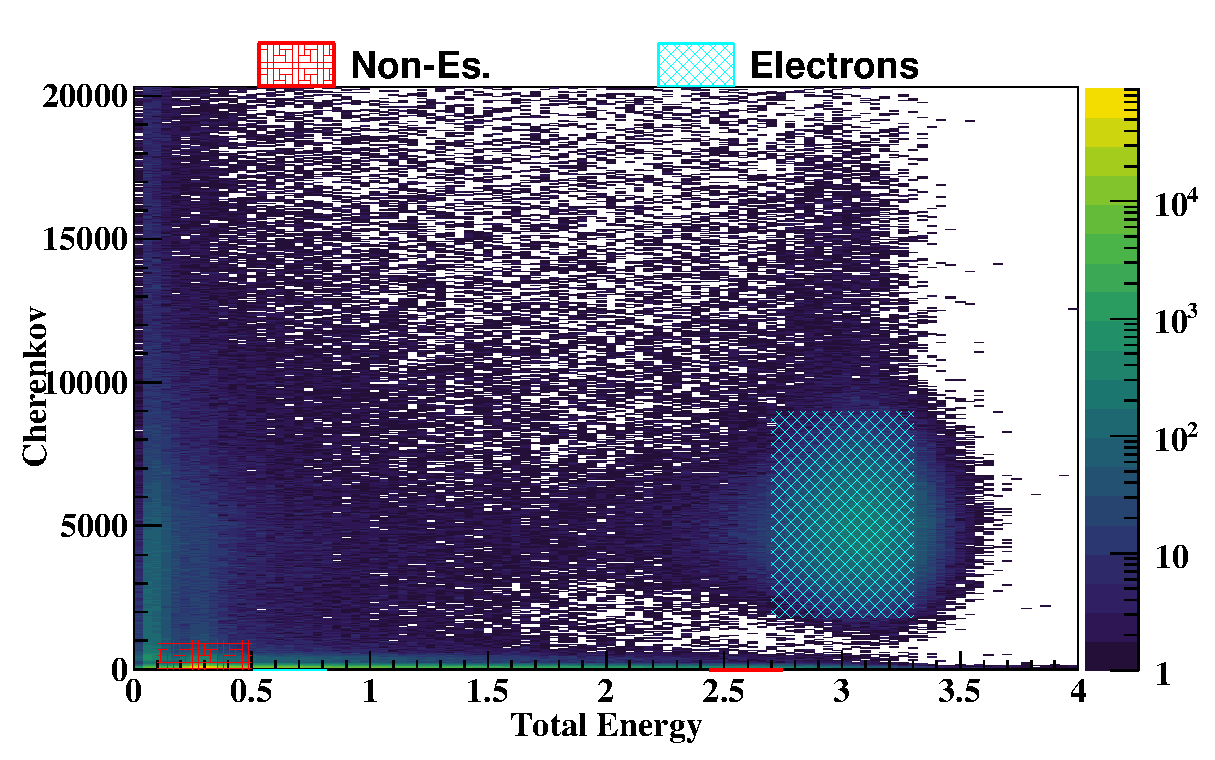
\includegraphics[width=13cm]{PID_2d}
	\caption{Two dimensional plot of the cherenkov sum versus Total Energy deposited, including electron sampling in teal and non-electron sampling in red. }
	\label{elesample}
\end{figure}

\begin{equation}\label{effequ}
\begin{split}
		GE_{sample} & = \textrm{Known electron sample from tight cut}  \\
	      GE_{pass} & = \textrm{$GE_{sample}$ and pass indentification cut} \\
	Electron_{eff}  & = \frac{ GE_{pass} } { GE_{sample} } 
\end{split}
\end{equation}
\paragraph{}The efficiency of the spectrometer's particle identification(PID) detectors was determined by using the first calorimeter layer, the second calorimeter layer, and the cherenkov to provide a samples of good electrons and other particles. The PID efficiency of the individual detectors were determined using equation \ref{effequ}. The good electron sample for calculating the efficiency of the single detector was defined by sampling through the other two detectors. Sampling through the two layers of the calorimeter is shown in figure \ref{Prl1Prl2}. The cherenkov good electron sample shown in figure \ref{cersam}. The electron sample from the cherenkov is contaminated by delta particles that are created by secondary scattering events from pions and a combination of unknown particles titled $X1$. The $X1$ events do not deposit enough energy into the calorimeter system to be consider as good electrons that scatter from our target. Using sampling in one layer of the calorimeter and the cherenkov, these unwanted low energy particles are rejected from sampling for efficiency calculations. 


\begin{figure}[]
{\centering
\textbf{Particle ID and efficiency sampling for the two layers of the calorimeter }\par\medskip}
\includegraphics[width=8.5cm]{Lplr1}
\includegraphics[width=8.5cm]{Lprl2}
\caption{Electrons and other back ground particles identified via cuts in the total calorimeter and the gas cherenkov shown in the individual layers of the calorimeters. Sampling cuts for Electrons in teal and Non-Electrons in red.}
\label{Prl1Prl2}
\end{figure}

\begin{figure}[]
{\centering
\textbf{Particle ID and efficiency sampling for Cherenkov }\par\medskip}
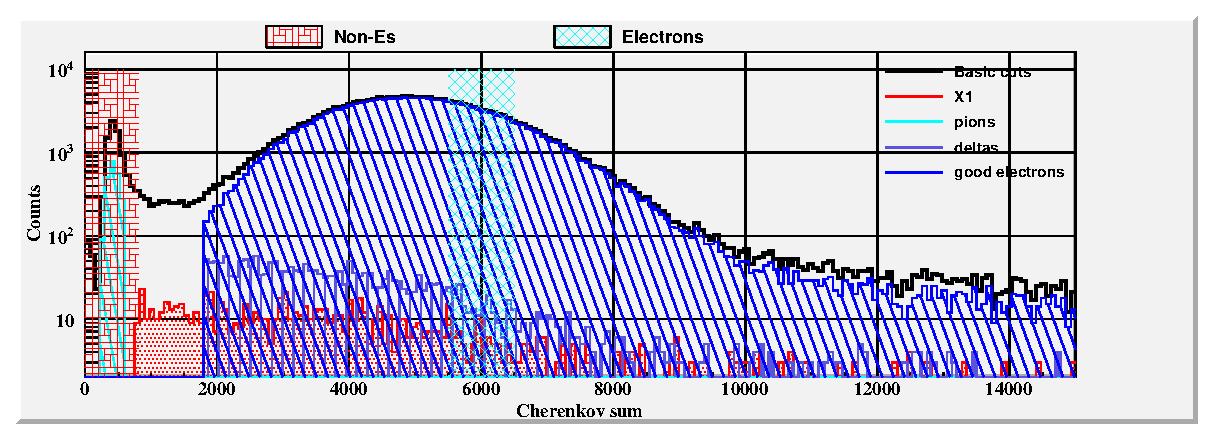
\includegraphics[ width=17cm]{Lcerasum}
\caption{Electrons and other back ground particles identified via cuts in the total calorimeter and the gas cherenkov shown in the sum of the gas cherenkov.Sampling cuts for Electrons in teal and Non-Electrons in red.}
\label{cersam}
\end{figure}

    	
\chapter{Results}
\paragraph{}The culminating part of this nuclear physics analysis begins with the extraction of the experimentally measured DIS cross sections for three targets. Then using those cross sections to study the per nucleon scaled A/D ratio. I will also use these A/D ratios to study the EMC effect for both $^3$He and $^3$H. In this chapter, I will present my results for the DIS cross sections and EMC effect. I will also discuss an error analysis for both the cross section measurements and the EMC effect results. 
\section{DIS Cross Section}
\paragraph{}Using the Monte Carlo ratio method, I extracted the experimental measured cross section for $^3$He, $^3$H, and $^2$D. These DIS cross section extraction ranges from 0.18 to 0.82 in $x$, from 2.2 to 11.8 GeV$^2$ in $Q^2$, and has W$^2$ $>3.5$ GeV$^2$. The central momentum setting of the spectrometer was 3.1 GeV/c and the spectrometer was moved from 17.5 to 33.5 degrees.


\begin{equation}
\sigma_{Data} = \sigma_{model} \cdot \frac{Y_{Data}}{Y_{MC}}. \nonumber
\end{equation}

%\iffalse
%\begin{landscape}
%\begin{sidewaysfigure}
\begin{figure}[t!]
	\hspace{-20pt}
	\includegraphics[width=17cm]{../images/total_xs.pdf}
	\caption{Experimentally measured cross section using the Monte Carlo ratio method for $^3$H, $^3$He, and $^2$D. Normalization uncertainty due to target thickness uncertainty for $^3$H= 0.97\%, $^3$He = 1.12\%, and $^2$D = 0.56\%.}
    \label{CCplot}
\end{figure}
%\end{sidewaysfigure}
%\end{landscape}
%\fi

\iffalse
\begin{landscape}
%\begin{sidewaysfigure}
\begin{figure}
	\hspace{-40pt}
	\includegraphics[width=27cm]{../images/total_xs_L.pdf}
	\caption{Experimentally measured cross section using the Monte Carlo ratio method for $^3$H, $^3$He, and $^2$D. Normalization uncertainty due to target thickness uncertainty for $^3$H= 0.97\%, $^3$He = 1.12\%, and $^2$D = 0.56\%.}
%label{CCplot}
\end{figure}
%\end{sidewaysfigure}
\end{landscape}
\fi


I compared the data yield to the Monte Carlo yield to produce a correcting factor for the model cross section. Figure \ref{D_MC_COMP} shows the ratio comparison between data and Monte Carlo in bins of $x$. Then apply the ratio factor for a bin in $x$ to the model cross section to extract out the experimentally measured cross section for that bin. Figure \ref{CCplot} shows a plot of the experimentally measured cross section for $^3$H, $^3$He, and $^2$D.  This is the first result of an inclusive DIS cross section for $^3$H and expands on the DIS cross section for $^3$He, pushing the invariant mass past the resonance region at higher values of $x$.  Appendix \ref{A_cst} contains tables of the cross section and summaries of the errors included in the error study for the cross section analysis of each target. 
\section{Cross Section Error Analysis}
\paragraph{}The measurement of the cross section requires finally tune detectors and analysis processes. Uncertainties arise due to the nature and limitations of the spectrometers and the analysis of the data received. In this section, I will discuss the calculation and propagation of errors in the analysis of the DIS cross section. The error analysis will be broken into the calculation of normalized yield for data, yield for Monte Carlo, and the model used for cross section extraction. Table \ref{ET_sum} contains the summary of the errors for the cross section extraction for the error on the yield, MC, and model. 

\begin{table}[]
	\caption{Relative Error Contributions for Cross Section for a selection of bins. This table contains the summary of relative error to the cross section for the yield, Monte Carlo, and Cross Section Model. Then summed in quadrature is the total relative error for the cross section.}
	\label{ET_sum}
\begin{tabular}{|l|l|l|l|l|l|l|}
	\hline
	\multicolumn{1}{|r|}{Xbjc}        & \textbf{0.185} & \textbf{0.305} & \textbf{0.49} & \textbf{0.57} & \textbf{0.705} & \textbf{0.825} \\ \hline
	Corrected Norm. Yield Error       & 0.01           & 0.01           & 0.014         & 0.015         & 0.014          & 0.016          \\ \hline
	MC and Model Total Error & 0.015          & 0.015          & 0.013         & 0.014         & 0.028          & 0.026          \\ \hline
	Cross Section Error               & 0.018          & 0.018          & 0.019         & 0.021         & 0.031          & 0.031          \\ \hline
\end{tabular}
\end{table}

\subsection{Normalized Yield Error}
\subsubsection{Corrected Electron Count Error}
\begin{align}
\dfrac{d\sigma}{dE^{\prime}d\Omega} &= \frac{(N - BG)}{\mathscr{L} \cdot \epsilon \cdot \Delta E^{\prime} \Delta \Omega \cdot A(E^{\prime},\theta)}. \nonumber\\
\sigma &= \text{NormY}/\left(\Delta E^{\prime} \Delta \Omega \cdot A(E^{\prime},\theta)\right)\nonumber\\
\text{NormY} &= \left(N_e \cdot BG/\epsilon \right) / \mathscr{L}
\end{align}

\paragraph{}
The contributions for error on the measurement of the normalized yield(normY) can be simplified into the contributions for the corrected number of electrons and the luminosity. The error for the corrected number of counted electrons includes the random statistical error for the count of electrons detected, the error associated with the calculated efficiencies, and the error from the background correction. The electron statics range from 4875 to more than 42000 in a bin and therefore I have treated the randomness of the counting in a standard error technique. The relative statistical error for a bin is $\frac{1}{\sqrt{Ne}}$ and ranges from .5\% to 1.4\%. Calculating the efficiencies deals with calculating a probability of a binomial choice. The errors associated with the efficiencies are calculated using the Wilson score interval described in equation \ref{WSI}, where $p$ is the efficiency or a probability of a success, $n$ is the number of samples, $z$ is 1.645 for a 95\% confidence level. 
\begin{equation}
p[_{UpperBound},_{LowerBound}] = \frac{ 2np +z^2 \pm \left[z\sqrt{z^2 - \frac{1}{n} + 4np(1-p) +(4p-2)} + 1 \right]}{2(n+z^2)} \label{WSI}
\end{equation}
The relative efficiency errors are added in quadrature to calculate an over all efficiency error to be propagated into the yield calculation.
\paragraph{}The correction for background events corrects for events from the end caps and pair produced electrons. The end cap correction factor is produced by a ratio of yields between the gas cells and the empty cell. This yield measurement allows for the cancellation of many of the systematic uncertainties. The largest contribution to the this error is the low statistics of the back ground events. The estimated error to the cross section analysis is about 1\%. Further study of the end cap contamination and the error associated with the correct is part of the ongoing analysis. The error for the positron correction involves using the covariance matrix for the exponential fit and propagating the error for each parameter of each target using the $x_{Bj}$ dependent function. The error for the fit parameters are propagated to an error for the correction using equation \ref{cv_err}.
\begin{equation}
\frac{\Delta f(x)}{f(x)} =  \sqrt{ \sum_{i}^{} \left(\delta p_i\cdot x^i\right)^2 + \sum_{ij}^{}\left( 2\cdot \delta p_{ij}\cdot \dfrac{df(x)}{dp_i}\cdot \dfrac{df(x)}{dp_i}\right) } \label{cv_err}
\end{equation}
The error for the background corrections are added in quadrature to get an overall error for the total back ground correction.  
\subsubsection{Luminosity Error}
\paragraph{}The errors involved in the luminosity calculated is the target density thickness measurement, beam charge calculation, and density correction. The error in the target thickness measurement is considered an overall normalization uncertainty. The error for the three gas targets' thickness measurements are: $^3$H= 0.97\%, $^3$He = 1.12\%, and $^2$D = 0.56\% \cite{HATT_eng}. The measurement uncertainties for each gas target are displayed in table \ref{tgt_table}. The amount of beam charge deposited on the target is calculated via the BCM(beam charge monitors) and their calibrations. The BCM calibrations were determined a few times through the run period with no change to the calibration constants. Due to the consistency of the BCMs and the high quality calibration the  error estimation for charge calculation is approximately 0.2\%. The error for the density correction is based in the error from the 2nd order polynomial fit. The error is calculated using the same method as the positron background correct, combining the errors for the fit parameters and the covariance terms through the propagation formula \ref{cv_err} using the current dependent correction function, \ref{eq:dc}. The relative error in charge on target and density correction have been added in quadrature to calculate a systematic error for the luminosity calculation. The systematic error for the luminosity and the systematic error for the correct count of electrons are then added in quadrature to calculate and overall normalized yield error.  
\begin{table}[]
	\caption{This table provides a summary of the error analysis for the Corrected Normalized Electron Yield. Containing the relative error for the bin statistics, background subtraction, efficiencies, and luminosity calculation. Including the total error on the Yield analysis for a selection of bins over the entire range of kinematics.  }
	\label{Y_Etable}
	\begin{tabular}{|l|l|l|l|l|l|l|}
		\hline
		\multicolumn{1}{|r|}{\textbf{Xbjc}} & \textbf{0.185} & \textbf{0.305} & \textbf{0.49} & \textbf{0.57} & \textbf{0.705} & \textbf{0.825} \\ \hline
		Stat Err                            & 0.0062         & 0.0053         & 0.0097        & 0.0106        & 0.011          & 0.0143         \\ \hline
		Density Correction             & 0.002          & 0.0024         & 0.003         & 0.003         & 0.0026         & 0.002          \\ \hline
		Positron Correction            & 0.0004         & 0.0002         & 0.0001        & 0.0001        & 0.0001         & 0.0001         \\ \hline
		End Cap Subtraction            & 0.007          & 0.007          & 0.007         & 0.007         & 0.0070         & 0.007          \\ \hline
		Efficiencies Error             & 0.004          & 0.0051         & 0.0075        & 0.0071        & 0.0041         & 0.0032         \\ \hline
		Corrected Norm. Yield Error    & 0.0104         & 0.0104         & 0.0145        & 0.0148        & 0.0139         & 0.0164         \\ \hline
	\end{tabular}
\end{table}

\subsection{Monte Carlo Yield Error}
\paragraph{}The responsibility of the Monte Carlo is to accurately account for the acceptance of the spectrometers. The uncertainty for thee Monte Carlo yield combines the statical uncertainty of the number of events generated and the reconstruction of the momentum and angle.  The statistical uncertainty is reduced due to the generation of a few million events. The uncertainty in the reconstruction of an event is a mixture of the uncertainties in the beam x and y position, spectrometer offsets, beam energy, optics, and acceptance cuts. The uncertainties for the beam x and y position was controlled by the BPMs and the calibration I completed. The uncertainty for the BPM measurements is 140 $\mu$m. The beam energy measurement is quoted to have an absolute accuracy of 5 x 10$^{-4}$.  The optics are capable of determining the relative in-plane angle with an accuracy of $\pm$ 0.2 mrad, out-of-plane angle with $\pm$ 0.6 mrad in the target coordinates, and momentum reconstruction 2.5x10$^{-4}$\cite{HallA}.  Using equation \ref{scatangle}, I propagated the resolution of target reconstruction variables to determine the relative uncertainty of the scattered angle to be $\approx$ 0.15\%. I have calculated the effect of the accuracy of the optics by comparing the cross section for the nominal values of , beam energy, scattered angle, and momentum, to the cross section of these values shifted by their uncertainties. A summary of the uncertainties used in the uncertainty of optics reconstruction are listed below. In table \ref{MC_ErrT}, I summary the relative errors associated the Monte Carlo yield and the model cross section discussed in the next section. 
\begin{itemize}
\item$\delta \theta$ = 0.15\%
\item$\delta E^{\prime}$ = $\pm$0.00025
\item$\delta E_{beam}$ = $\pm$0.0005
\end{itemize}
Using the errors in scattering angle, scattering momentum, and beam energy, I calculated an approximate error associated with the reconstruction events into $x$ bins with equation \ref{reconErr}. The fluctuation of this error is large and ranges from 1/2\% to 1.5\% and therefore will be applied on a point to point bases. 

\begin{equation}
\frac{\Delta \sigma(E,E^{\prime},\theta)}{ \sigma(E,E^{\prime},\theta)} = \frac{\sigma(E+\Delta E_{beam},E^{\prime}+\Delta E^{\prime},\theta+\Delta \theta) - \sigma(E,E^{\prime},\theta)}{\sigma(E,E^{\prime},\theta)} \label{reconErr}
\end{equation}

\subsection{Cross Section Model Error}
\paragraph{}
The model dependence of the DIS cross section and the radiative corrections are the two factors of the systematic error that accompanies the Monte Carlo ratio method. My analysis of the model depended errors used different DIS cross section models to supply an error for the model cross section and the radiative corrections. The models I will used to study the model dependent error can be broken into 3 sections, models for F$_{2d}$, model for EMC correction, and model for the ratio for $F_{2n}/F_{2p}$. I will two models to form the $^2$D structure function Ari Bodek \cite{DISmodel} and M. Arneodo's NMC model \cite{NMC_model}. I will use two EMC correction models, Kulagin, S. A. and Petti, R. \cite{kpmodel}, and a SLAC EMC correction \cite{SLAC_bodek}. The structure function ratio is formed by two models also, linear Ratio = (1 - 0.8$*x$) and NMC \cite{NMC_ratio}. The model depended error was estimated by comparing the different models together with the chosen model. In the extreme case, this error reached a maximum of 2\%    
\begin{table}[]
	\caption{This table contains a summary of the relative error for the Monte Carlo yield extraction and the model cross section. Also, I include the errors add in quadrature for these two analysis parts. }
	\label{MC_ErrT}
	\begin{tabular}{|l|l|l|l|l|l|l|}
		\hline
		\multicolumn{1}{|r|}{\textbf{Xbjc}} & \textbf{0.185} & \textbf{0.305} & \textbf{0.49} & \textbf{0.53} & \textbf{0.705} & \textbf{0.825} \\ \hline
		MC Stat Error                           & 0.003          & 0.002          & 0.003         & 0.002         & 0.002          & 0.002          \\ \hline
		Resolution Error                       & 0.015          & 0.011          & 0.006         & 0.004         & 0.007          & 0.02           \\ \hline
		Model Error                    & 0.002          & 0.01           & 0.011         & 0.011         & 0.027          & 0.018          \\ \hline
		MC and Model Total Error   & 0.015          & 0.015          & 0.013         & 0.012         & 0.028          & 0.026          \\ \hline
	\end{tabular}
\end{table}

\section{EMC Ratios}
\paragraph{}In this section, I will present the A/D cross section ratios for $^3$He and $^3$H. The ratios are normalized by the number of nucleons in each target. Included in figure \ref{ADplot} are results from E03103. These results have different invariant mass but are considered DIS until 0.65 in $x$. Above this threshold, the invariant mass begins to drop lower then the DIS criteria used for my analysis. 
%\begin{landscape}
%\begin{sidewaysfigure}
%\thispagestyle{empty}
%\raisebox{-14.5cm}{\makebox[\linewidth]{\thepage}}
\begin{figure}
	\centering
	\includegraphics[width=15.5cm]{../images/A_D_ratios.pdf}
	\caption{The A/D ratio for $^3$He and $^3$H from my analysis. Also included, EMC analysis from E03103\cite{seeley} and the EMC ratios from a DIS scattering model from Arie Bodek model \cite{DISmodel}.}
	\label{ADplot}
\end{figure}

%\end{sidewaysfigure}
%\end{landscape}

\subsection{Isoscalar Correction}
	\paragraph{}The definition of an EMC effect ratio is the ratio of the per nucleon cross section ratio of a target nucleus with $^2$D. Also,  this comparison is of a target with equal number of protons and neutrons, an isoscalar nuclei. When looking at the EMC ratio of a target with not an equal number of nucleons, an isoscalar correction needs to be applied. This correction is used to correct for the difference in cross section between the neutron and proton. The per nucleon nuclear F$_2^A $ of an unsymmetrical nucleon can be written as:
	\begin{equation}
	\frac{1}{A}\left(ZF^p_2 + \left(A-Z\right)F^2_n\right)\nonumber
	\end{equation}
	and a symmetrical nucleon can be simplified to:
	\begin{equation}
		\frac{1}{2}\left(F^p_2 + F^2_n\right).\nonumber
	\end{equation}	
	The isoscalar correction can be determine by applying a correction function $f_{iso}$ to equate the two previous equations and solving that combination for the correction function.
	\begin{equation}
		\frac{1}{2}\left(F^p_2 + F^2_n\right) =  f^A_{iso}\frac{1}{A}\left(ZF^p_2 + \left(A-Z\right)F^2_n\right)\nonumber
	\end{equation}
	\begin{equation}
	f^A_{iso} = \frac{\frac{1}{2}\left(1+F^n_2/F^p_n\right)}{\frac{1}{A}\left(Z +(A-Z)F^n_2/F^p_n\right)} \label{isoC}
	\end{equation}
	\paragraph{}The isoscalar correction for a nuclear target depends on A,Z, and the F$_2$ ratio. There exist no data on the free neutron, so the $F^n_2/F^p_n$ is a model dependent extraction. The  F$_2$ ratio has been extracted from the ratio of $^3$H to $^3$He from the MARATHON experiment and $^2$D to hydrogen ratios from previous experiments from SLAC and the NMC. I have used the $F^n_2/F^p_n$ from MARATHON to calculate my iscscalar correction for both $^3$He and $^3$H. I have estimated the error of this model dependent correction by comparing the isoscalar correction from the MARATHON extraction with the isoscalar correction using three other $F^n_2/F^p_n$ models Kulagin, S. A. and Petti, R. \cite{kpmodel}, J. Arrington \cite{JA_FR}, and NMC \cite{NMC_ratio}. The relative variance of this calculation ranges from $\pm$ 0.1\% to $\pm$ 3.8\% for $^3$H EMC ratio. These 4 models and the error band from this study is shown in figure \ref{isofuncs} for the isoscalar correction on $^3$H and figure \ref{isofuncsHe3} for the isoscalar correction on $^3$He.

	\begin{figure}[!]
		\includegraphics[width=15cm]{ISOfacsH3.pdf}
		\caption{Isoscalar correction factor for the $^3$H EMC ratio from four different models discussed in this section.}
		\label{isofuncs}
		\vspace{1cm}
		\includegraphics[width=15cm]{ISOfacsHe3.pdf}
		\caption{Isoscalar correction factor for the $^3$He EMC ratio from four different models discussed in this section.}
		\label{isofuncsHe3}
	\end{figure}

\section{EMC Effect}
\paragraph{} Using the extracted cross section of the two A=3 nuclei and $^2$D, the first measurement of the $^3$H EMC effect has been achieved. The data also provides a comparison of the EMC effect of the mirror nuclei $^3$He. MARATHON's design of rotating targets, and uniform data taking procedure allows for the cancellation of the detector efficiency correction factors and corrections due to acceptance issues. This will reduce the size of the uncertainty of the EMC effect measurement and provides precise result for the EMC ratio of the two A=3 nuclei. 
\paragraph{}The isoscalar corrected EMC Effect ratios for $^3$He and $^3$H from my inclusive DIS cross section extraction are displayed in figures \ref{ISOEMC_He3} and \ref{ISOEMC_H3}. These results provide a comparison between my extract of the $^3$He EMC and the $^3$He EMC results from the E03103 from J. Seeley and A. Daniels \cite{seeley}. My EMC effect for $^3$He shows good agreement with the E03103 experimental results within uncertainty. The EMC results are plotted with error bars that represent the total point to point uncertainty for the EMC measurement and an error band for the overall normalization uncertainty dominated by the error in target thickness measurement.  
	\begin{figure}[!]
		\includegraphics[width=15cm]{EMCIsoHe3.pdf}
		\caption{Isoscalar corrected EMC ratio for $^3$He. The point to point error bars are the total systemic and statical errors for the EMC effect.}
		\label{ISOEMC_He3}
	\vspace{1cm}
	\includegraphics[width=15cm]{EMCIsoH3.pdf}
	\caption{Isoscalar corrected EMC ratio for $^3$H. The point to point error bars are the total systemic and statical errors for the EMC effect.}
	\label{ISOEMC_H3}
\end{figure}

\subsection{Ratio of EMC Effects}
\paragraph{} If figure \ref{ISORatio}, I display the results of the ratio of the two A=3 mirror nuclei EMC effects. The errors associated with the extraction of this ratio are the errors for extracted both cross sections and the errors for the ratio of the isoscalar correction. For the errors on the isoscalar correction, I looked at the ratio of isoscalar correction for the different models and extracted the standard deviation from the model dependence on the ratio. The error bars in figure \ref{ISORatio} are all error contributions added in quadrature. 

\begin{figure}
	\includegraphics[width=15cm]{Iso_H_He.pdf}
	\caption{Ratio of the isoscalar corrected  $^3$H EMC Effect and $^3$He EMC Effect.}\label{ISORatio}
\end{figure}

    	
\chapter{Conclusion}
\paragraph{}The MARATHON experiment took inclusive DIS data on the special designed sealed tritium cells, filled with tritium, helium, and deuterium at JLab. The unique opportunity provided by access of tritium allowed the MARATHON experiment to be the first to use DIS to study the internal structurer of this radioactive A=3 system. Alongside tritium, DIS data was taken on both helium-3 and deuterium. The experimental kinematics produces DIS events for $x$ from 0.18 to 0.8, with a Q$^2$ range of 3 to 12 (GeV$^2$) by rotating the electron spectrometer from 17.5 to 36 degrees and using CEBAF's 10.6 GeV beam. 
\paragraph{}The MARATHON data was used to produce the inclusive DIS cross section for these three gas targets. This measurement has provided the first extraction of the DIS cross section for tritium. Using the cross section measurements of the two A=3 mirror nuclei and deuterium, the MARATHON collaboration has calculated the A=3 EMC effect for both helium-3 and tritium. This experiment will provide the first ever results on the EMC effect of tritium and the first  on the comparison of the EMC effects of the two A=3 mirror nuclei.
\paragraph{}
    %%%%%%%%%%%%%%%%%%%%%%%%%%%%%%%%%%%%%%%%%%%%%%%%%%%%%%%%%%%%%%%%%%%%%%%%%%%%%%%%%%%%%%%%%%%%%%%%%%%%%
    % BIBLIOGRAPHY
    %%%%%%%%%%%%%%%%%%%%%%%%%%%%%%%%%%%%%%%%%%%%%%%%%%%%%%%%%%%%%%%%%%%%%%%%%%%%%%%%%%%%%%%%%%%%%%%%%%%%%
    \makeBibliographyPage % make the bibliography title page
\newpage

% To make the bibliography, use \utbiblio{#1}{}{} command. Always use "#1" for the first entry. The second entry is your bibliography style, and the third entry is the name of your bibliography file (.bib file extension) 
% bibliography style - recommend using apalike-doi as it hyperlinks DOIs
% Be sure to run BibTeX in order to generate the bibliography correctly.

%\utbiblio{#1}{apalike}{references/references-dissertation}


%\makeBibliographyPage % make the bibliography title page - can be edited in ut-thesis-template.tex
\begingroup
\def\chapter*#1{}
\bibliographystyle{plain} %plain bibliography style - recommend using apalike-doi as it hyperlinks DOIs
\bibliography{references/references-dissertation} % references.bib included in the references directory
\endgroup
%%%%%%%%%%%%%%%%%%%%%%%%%%%%%%%%%%%%%%%%%%%%%%%%%%%%%%%%%%%%%%%%%%%%%%%%%%%%%%%%%%%%%%%%%%%%%%%%%%%%%
% APPENDIX - OPTIONAL - COMMENT OUT IF NOT NEEDED
%%%%%%%%%%%%%%%%%%%%%%%%%%%%%%%%%%%%%%%%%%%%%%%%%%%%%%%%%%%%%%%%%%%%%%%%%%%%%%%%%%%%%%%%%%%%%%%%%%%%%

\makeAppendixPage{2}   % Input the number of appendices
\appendix    
\chapter{Cross Section Tables}\label{CST}
\paragraph{}This appendix contains the cross section tables for the three gas targets, $^3$H, $^3$He, and D. The data used to produce the cross section for these targets was acquired during the MARATHON experiment completed at JLab. The error for the three gas targets' thickness measurements are: $^3$H= 0.97\%, $^3$He = 1.12\%, and $^2$D = 0.56\% \cite{HATT_eng}.  The cuts used to produce the tables:

\textbf{Electron Selection Cuts}\\
\begin{tabular}{@{$\bullet$ }lll}
	-0.07 m &$>=$& Vertex Z $<=$ 0.09 m\\
	-0.035 &$ >=$ &$\delta_{tg} <=$ -0.035\\
	-0.04 rad &$>=$  &$\theta_{tg} <=$ -0.04 rad\\
	-0.025 rad &$>=$  &$\phi_{tg}   <=$ -0.025 rad\\
	Number of tracks & ==& 1\\
	MARATHON trigger (bit)  &\& &(1$<<$2)\\
	Total Cherenkov ADC sum &$>$ &1800\\
	Calo. Layer 1 Energy &$>$ & 1 GeV\\
	Calo. Layer 2 Energy &$>$ & 0.6 GeV\\
		W$^2$ &$>$ &2.5
\end{tabular}

\pagebreak
\newgeometry{hmargin=1in,vmargin=1in}
\thispagestyle{lscape}
\pagestyle{lscape}
\begin{landscape}

\begin{table}	
%\begin{sidewaystable}
\centering
\caption{Cross section table for $^3$H. }\label{CST_H3}
	\begin{tabular}{|p{1cm}|p{1cm}|p{1.5cm}|p{1.5cm}|p{2cm}|p{2cm}|p{1.5cm}|p{1.5cm}|p{2.5cm}|p{2.5cm}|}
		\hline
		x     & Q2     & Cross Section & Stat. Error & Density Cor. & Positron Sub. & Endcap Sub. & Detector Eff. & MC \& Model Error & Cross Section Error \\ \hline
		0.185 & 2.708  & 18.776        & 0.0055            & 0.002              & 0.0004               & 0.007              & 0.004                 & 0.016             & 0.019               \\ \hline
		0.215 & 3.055  & 15.49         & 0.0045            & 0.002              & 0.0002               & 0.007              & 0.004                 & 0.014             & 0.017               \\ \hline
		0.245 & 3.446  & 11.996        & 0.0049            & 0.002              & 0.0002               & 0.007              & 0.0041                & 0.013             & 0.016               \\ \hline
		0.275 & 3.881  & 8.617         & 0.0051            & 0.002              & 0.0001               & 0.007              & 0.0045                & 0.014             & 0.017               \\ \hline
		0.305 & 4.311  & 6.28          & 0.0059            & 0.002              & 0.0002               & 0.007              & 0.0051                & 0.014             & 0.018               \\ \hline
		0.335 & 4.705  & 4.931         & 0.0073            & 0.002              & 0.0002               & 0.007              & 0.0057                & 0.014             & 0.018               \\ \hline
		0.365 & 5.122  & 3.767         & 0.0082            & 0.002              & 0.0002               & 0.007              & 0.0067                & 0.014             & 0.019               \\ \hline
		0.395 & 5.55   & 2.794         & 0.0098            & 0.002              & 0.0002               & 0.007              & 0.0079                & 0.013             & 0.02                \\ \hline
		0.425 & 6.023  & 2.049         & 0.0091            & 0.002              & 0.0001               & 0.007              & 0.0091                & 0.013             & 0.02                \\ \hline
		0.455 & 6.397  & 1.591         & 0.009             & 0.002              & 0.0001               & 0.007              & 0.0091                & 0.013             & 0.02                \\ \hline
		0.49  & 6.922  & 1.153         & 0.01              & 0.002              & 0.0001               & 0.007              & 0.0083                & 0.013             & 0.02                \\ \hline
		0.53  & 7.472  & 0.776         & 0.0086            & 0.002              & 0.0001               & 0.007              & 0.0075                & 0.014             & 0.019               \\ \hline
		0.57  & 8.045  & 0.527         & 0.0111            & 0.002              & 0.0001               & 0.007              & 0.0071                & 0.016             & 0.022               \\ \hline
		0.61  & 8.617  & 0.351         & 0.0102            & 0.002              & 0.0001               & 0.007              & 0.0064                & 0.02              & 0.024               \\ \hline
		0.655 & 9.241  & 0.22          & 0.0115            & 0.002              & 0.0001               & 0.007              & 0.0055                & 0.025             & 0.029               \\ \hline
		0.705 & 9.997  & 0.121         & 0.0113            & 0.002              & 0.0                  & 0.007              & 0.0041                & 0.03              & 0.033               \\ \hline
		0.76  & 10.688 & 0.065         & 0.0109            & 0.002              & 0.0                  & 0.007              & 0.0035                & 0.026             & 0.029               \\ \hline
		0.825 & 11.468 & 0.03          & 0.0143            & 0.002              & 0.0                  & 0.007              & 0.0032                & 0.037             & 0.04                \\ \hline
	\end{tabular}
\end{table}
%\end{sidewaystable}
\end{landscape}
\restoregeometry
\pagestyle{plain}

\pagebreak
\newgeometry{hmargin=1in,vmargin=1in}
\thispagestyle{lscape}
\begin{landscape}

	\begin{table}
			\centering
	\caption{Cross section table for $^3$H.}\label{CST_He3}
	\begin{tabular}{|p{1cm}|p{1cm}|p{1.5cm}|p{1.5cm}|p{2cm}|p{2cm}|p{1.5cm}|p{1.5cm}|p{2.5cm}|p{2.5cm}|}
	\hline
	x     & Q2     & Cross Section & Stat. Error & Density Cor. & Positron Sub. & Endcap Sub. & Detector Eff. & MC \& Model Error & Cross Section Error \\ \hline
		0.185 & 2.709  & 20.71         & 0.0063            & 0.002              & 0.0006               & 0.007              & 0.004                 & 0.016             & 0.019               \\ \hline
		0.215 & 3.059  & 17.303        & 0.0051            & 0.002              & 0.0004               & 0.007              & 0.004                 & 0.015             & 0.018               \\ \hline
		0.245 & 3.447  & 13.59         & 0.0052            & 0.002              & 0.0002               & 0.007              & 0.0041                & 0.016             & 0.019               \\ \hline
		0.275 & 3.88   & 9.842         & 0.0056            & 0.002              & 0.0002               & 0.007              & 0.0044                & 0.017             & 0.02                \\ \hline
		0.305 & 4.313  & 7.22          & 0.0064            & 0.002              & 0.0002               & 0.007              & 0.0051                & 0.017             & 0.02                \\ \hline
		0.335 & 4.708  & 5.803         & 0.0074            & 0.002              & 0.0002               & 0.007              & 0.0058                & 0.017             & 0.021               \\ \hline
		0.365 & 5.122  & 4.446         & 0.0081            & 0.002              & 0.0002               & 0.007              & 0.0067                & 0.016             & 0.02                \\ \hline
		0.395 & 5.549  & 3.419         & 0.0095            & 0.002              & 0.0002               & 0.007              & 0.0079                & 0.015             & 0.021               \\ \hline
		0.425 & 6.024  & 2.499         & 0.009             & 0.002              & 0.0002               & 0.007              & 0.0091                & 0.014             & 0.02                \\ \hline
		0.455 & 6.397  & 1.974         & 0.0089            & 0.002              & 0.0002               & 0.007              & 0.0091                & 0.013             & 0.02                \\ \hline
		0.49  & 6.924  & 1.434         & 0.0098            & 0.002              & 0.0001               & 0.007              & 0.0083                & 0.012             & 0.019               \\ \hline
		0.53  & 7.473  & 0.985         & 0.0083            & 0.002              & 0.0001               & 0.007              & 0.0075                & 0.011             & 0.017               \\ \hline
		0.57  & 8.044  & 0.668         & 0.0108            & 0.002              & 0.0001               & 0.007              & 0.0071                & 0.013             & 0.02                \\ \hline
		0.61  & 8.616  & 0.447         & 0.0099            & 0.002              & 0.0001               & 0.007              & 0.0064                & 0.017             & 0.022               \\ \hline
		0.655 & 9.242  & 0.282         & 0.0112            & 0.002              & 0.0001               & 0.007              & 0.0055                & 0.024             & 0.028               \\ \hline
		0.705 & 9.998  & 0.158         & 0.0111            & 0.002              & 0.0001               & 0.007              & 0.0041                & 0.033             & 0.036               \\ \hline
		0.76  & 10.689 & 0.087         & 0.0105            & 0.002              & 0.0                  & 0.007              & 0.0035                & 0.035             & 0.037               \\ \hline
		0.825 & 11.467 & 0.038         & 0.0141            & 0.002              & 0.0                  & 0.007              & 0.0031                & 0.024             & 0.029               \\ \hline
	\end{tabular}
	\end{table}
\end{landscape}

\restoregeometry
\pagestyle{plain}

\pagebreak
\newgeometry{hmargin=1in,vmargin=1in}
\thispagestyle{lscape}
\begin{landscape}

	\begin{table}
			\centering
	\caption{Cross section table for D.}\label{CST_D2}
	\begin{tabular}{|p{1cm}|p{1cm}|p{1.5cm}|p{1.5cm}|p{2cm}|p{2cm}|p{1.5cm}|p{1.5cm}|p{2.5cm}|p{2.5cm}|}
	\hline
	x     & Q2     & Cross Section & Stat. Error & Density Cor. & Positron Sub. & Endcap Sub. & Detector Eff. & MC \& Model Error & Cross Section Error \\ \hline
		0.185 & 2.708  & 13.048        & 0.0062            & 0.002              & 0.0004               & 0.007              & 0.004                 & 0.015             & 0.018               \\ \hline
		0.215 & 3.061  & 10.858        & 0.0051            & 0.002              & 0.0002               & 0.007              & 0.004                 & 0.013             & 0.016               \\ \hline
		0.245 & 3.452  & 8.473         & 0.0051            & 0.002              & 0.0002               & 0.007              & 0.0041                & 0.013             & 0.016               \\ \hline
		0.275 & 3.883  & 6.147         & 0.0049            & 0.002              & 0.0001               & 0.007              & 0.0045                & 0.014             & 0.017               \\ \hline
		0.305 & 4.31   & 4.596         & 0.0053            & 0.0024             & 0.0002               & 0.007              & 0.0051                & 0.015             & 0.018               \\ \hline
		0.335 & 4.695  & 3.724         & 0.0066            & 0.0027             & 0.0002               & 0.007              & 0.0055                & 0.015             & 0.019               \\ \hline
		0.365 & 5.119  & 2.812         & 0.0083            & 0.0033             & 0.0001               & 0.007              & 0.0064                & 0.015             & 0.02                \\ \hline
		0.395 & 5.549  & 2.111         & 0.0119            & 0.004              & 0.0001               & 0.007              & 0.0079                & 0.014             & 0.022               \\ \hline
		0.425 & 6.023  & 1.574         & 0.0115            & 0.003              & 0.0001               & 0.007              & 0.0091                & 0.014             & 0.022               \\ \hline
		0.455 & 6.397  & 1.279         & 0.0112            & 0.003              & 0.0001               & 0.007              & 0.0091                & 0.013             & 0.021               \\ \hline
		0.49  & 6.944  & 0.868         & 0.0113            & 0.003              & 0.0001               & 0.007              & 0.0081                & 0.013             & 0.021               \\ \hline
		0.53  & 7.474  & 0.615         & 0.0083            & 0.003              & 0.0001               & 0.007              & 0.0075                & 0.012             & 0.018               \\ \hline
		0.57  & 8.045  & 0.427         & 0.0106            & 0.003              & 0.0001               & 0.007              & 0.0071                & 0.014             & 0.02                \\ \hline
		0.61  & 8.615  & 0.286         & 0.0096            & 0.003              & 0.0                  & 0.007              & 0.0064                & 0.017             & 0.022               \\ \hline
		0.655 & 9.239  & 0.179         & 0.011             & 0.003              & 0.0                  & 0.007              & 0.0055                & 0.022             & 0.026               \\ \hline
		0.705 & 9.992  & 0.098         & 0.011             & 0.0026             & 0.0                  & 0.007              & 0.0041                & 0.028             & 0.031               \\ \hline
		0.76  & 10.688 & 0.052         & 0.0109            & 0.0022             & 0.0                  & 0.007              & 0.0035                & 0.027             & 0.03                \\ \hline
		0.825 & 11.467 & 0.023         & 0.0143            & 0.002              & 0.0                  & 0.007              & 0.0032                & 0.026             & 0.031               \\ \hline
	\end{tabular}
	\end{table}
\end{landscape}
\restoregeometry
\pagestyle{plain}
\include{back-matter/appendix-2}
%%%%%%%%%%%%%%%%%%%%%%%%%%%%%%%%%%%%%%%%%%%%%%%%%%%%%%%%%%%%%%%%%%%%%%%%%%%%%%%%%%%%%%%%%%%%%%%%%%%%%
% A VITA IS REQUIRED
%%%%%%%%%%%%%%%%%%%%%%%%%%%%%%%%%%%%%%%%%%%%%%%%%%%%%%%%%%%%%%%%%%%%%%%%%%%%%%%%%%%%%%%%%%%%%%%%%%%%%
\addToTOC{Vita}
% resume.tex
% vim:set ft=tex spell:



\setlength{\tabcolsep}{0em}



\lfoot{Jason Bane}


% indentsection style, used for sections that aren't already in lists
% that need indentation to the level of all text in the document
\newenvironment{indentsection}[1]%
{\begin{list}{}%
		{\setlength{\leftmargin}{#1}}%
		\item[]%
	}
	{\end{list}}

% opposite of above; bump a section back toward the left margin
\newenvironment{unindentsection}[1]%
{\begin{list}{}%
		{\setlength{\leftmargin}{-0.5#1}}%
		\item[]%
	}
	{\end{list}}

% format two pieces of text, one left aligned and one right aligned
\newcommand{\headerrow}[2]
{\begin{tabular*}{\linewidth}{l@{\extracolsep{\fill}}r}
		#1 &
		#2 \\
\end{tabular*}}

% make "C++" look pretty when used in text by touching up the plus signs
\newcommand{\CPP}
{C\nolinebreak[4]\hspace{-.05em}\raisebox{.22ex}{\footnotesize\bf ++}}

\begin{center}
{\large \textbf{Vita}}\\
{\large \textbf{Jason Bane}}

\end{center}

\hrule
\vspace{-0.4em}
\subsection*{Education}

\begin{itemize}
\parskip=0.1em

\item 
\headerrow
{\textbf{University of Tennessee}}
{\textbf{Knoxville, TN}}

\headerrow
{\emph{Ph.D. in Nuclear Physics}}
{\emph{August 2012 -- Planned December 2019}}
\headerrow
{\emph{Thesis: The EMC Effect in A=3 Nuclei}}
{\emph{Advisor: Nadia Fomin}}
%	\begin{itemize*}
%		\item Lorem ipsum dolor sit amet, consectetuer adipiscing elit.
%		\item Mirum est notare quam littera gothica, quam nunc putamus parum
%		claram.
%	\end{itemize*}


\parskip=0.1em

\item 
\headerrow
{\textbf{University of Tennessee}}
{\textbf{Knoxville, TN}}
\\
\headerrow
{\emph{Secondary Education Certification in}\\\emph{ Math and Science}}
{\emph{August 2009 -- May 2010}}
%	\begin{itemize*}
%		\item Lorem ipsum dolor sit amet, consectetuer adipiscing elit.
%		\item Mirum est notare quam littera gothica, quam nunc putamus parum
%		claram.
%	\end{itemize*}


\parskip=0.1em

\item 
\headerrow
{\textbf{University of Tennessee}}
{\textbf{Knoxville, TN}}
\\
\headerrow
{\emph{Bachelor of Science, Physics}\\ \emph{ \& Minor in Education }}
{\emph{August 2004 -- May 2009}}

%	\begin{itemize*}
%		\item Lorem ipsum dolor sit amet, consectetuer adipiscing elit.
%		\item Mirum est notare quam littera gothica, quam nunc putamus parum
%		claram.
%	\end{itemize*}

\end{itemize}
\hrule
\vspace{-0.4em}
\subsection*{Experience}

\begin{itemize}
\parskip=0.1em

\item
\headerrow
{\textbf{University of Tennessee}\\\textbf{Department of Physics and Astronomy }}
{\textbf{  Knoxville, TN,}}
\\
\headerrow
{\emph{Graduate Research Assistant }}
{\emph{May 2014 -- Present}}

\begin{itemize}[leftmargin=-.05in]
	\item Designed and constructed front end electronics for an electron spectrometer.
	\item Created module layouts and cable maps for efficient reuse of products.
	\item Tested high voltage cards and laid high voltage cable for an electron spectrometer.
	\item Used oscilloscopes to test signals, debug logic modules, and map out inconsistent signals.  
	\item Maintained and refurbished individual detector components of a spectrometer including checking the quality of Photo Multiplier Tubes and plastic scintillators.
	\item Calibrated detectors and used online analysis tools in Java to control the quality of data during shifts for an experiment. 
	\item Performed analysis on a large set of data involving multiple nuclear targets using Python, C++ , ROOT, and Fortran. 
	\item Worked with a diverse collaboration, leading projects and working as a team member
\end{itemize}
\vspace{0.85cm}
\item
\headerrow
{\textbf{University of Tennessee}\\\textbf{Department of Physics and Astronomy }}
{\textbf{  Knoxville, TN,}}
\\
\headerrow
{\emph{Graduate Teaching Assistant }}
{\emph{August 2012 -- May 2015}}
\begin{itemize}[leftmargin=-.05in]
	\item Designed and implemented observational and planetarium based astronomy labs.
	\item Educated students on the use of refracting telescopes and equatorial mounts.
	\item Instructed students in laboratory exercises to help conceptualize physics topics.
	\item Tutored students for homework assistance and test prep.
\end{itemize}
\begin{samepage}
	\item
	\headerrow
	{\textbf{Clay County Tennessee Education Department}}
	{\textbf{Celina, TN}}
	\\
	\headerrow
	{\emph{Secondary Educator \& Football Coach}}
	{\emph{August 2010 -- May 2012 }}
	\begin{itemize}[leftmargin=-.05in]	
		\item Created lesson plans that included interactive, creative thinking, and discussion driven curriculum for a diverse body of geometry students.
		\item Constructed lessons that used hands-on lab activities, demonstrations, and interactive computer lessons to instruct high school Juniors and Seniors in algebra-based physics. 
		\item Used discussion-based problem-solving lessons to help remedial math students to improve their algebra, geometry and trigonometry skills for post-secondary education. 
		\item Provided an equitable and inclusive atmosphere for diverse students. 
		\item Math and reading focused tutoring. 
	\end{itemize}
\end{samepage}
\end{itemize}




\hrule
\vspace{-0.4em}
\subsection*{Core Technical Skills}

\begin{indentsection}{\parindent}
\hyphenpenalty=1000
\begin{description}
	\item[Hardware:]
	Detector maintenance and wiring, front end electronics design and implementation, logical trigger design and testing   
	\item[Languages:]
	C, \CPP, \LaTeX, Python, shell script, SQL \\
	Monte Carlo Simulation Packages\\
	Example scripts located at https://github.com/jbane11/examples
	\item[Software:]
	Microsoft Office, Libre Office, Texstudio, vim, atom
	\item[Operating Systems:]
	Linux(Red Hat), Windows, MacOS
	
\end{description}
\end{indentsection}
\hrule
\subsection*{Publications}
\begin{itemize} \itemsep -2pt % Reduce space between items
\item  H. Dai, [et al. including \textbf{J. Bane}], ``First Measurement of the Ar(e,$e^\prime$)X Cross Section at Jefferson Lab," Phys. Rev. C 99, 054608 May 2019
\item R. Cruz-Torres, [et al. including \textbf{J. Bane}], ``Comparing proton momentum distributions in A=3 nuclei via $^3$He and $^3H$(e,$e^\prime$p) measurements," in preparation, (2019)
\item S. N. Santiesteban, S. Alsalmi, D. Meekins, \textbf{J. Bane,} et al., ``Density Changes in Low Pressure Gas Targets for Electron Scattering Experiments" NIM A 940, 2019
\item  H. Dai, [et al. including \textbf{J. Bane}], ``First Measurement of the Ti(e,$e^\prime$)X Cross Section at Jefferson Lab," Phys. Rev. C 98, 014617 July 2018
\item P V. Pandey, [et al. including \textbf{J. Bane}], ``Probing electron-argon scattering for liquid-argon based neutrino-oscillation program," preprint arXiv:1711.01671

\end{itemize}
\hrule
\subsection*{Honors}
\begin{itemize}
\item Jefferson Science Associates graduate fellowship award (2018)  
\item Chancellor’s honors for extraordinary professional promise (2016) 
\item DOE Office of Science Graduate Student Research program award (2015)
\item Dean's List 2009 Academic Year (2010)
\end{itemize}
\hrule
\subsection*{Conference Presentations}
\begin{itemize}
\item F$_2$ ratio and EMC effect for A=3 Mirror Nuclei", 24th European Conference on Few-body Problems in Physics, University of Surrey, England, September 2019.
\item "EMC in A=3 from MARATHON," 2nd Workshop on Quantitative Challenges in SRC and EMC Research,  MIT, Cambridge MA,  March 2019
\item "Ratios in A=3 nuclei from MARATHON ," American Physical Society's Division of Nuclear Physics' yearly meeting, HA, October 2018
\item "Measurement of the spectral function of Argon and Titanium through the(e,$e^\prime$p) reaction," American Physical Society's Division of Nuclear Physics' yearly meeting, HA, October 2018
\item "Status of the MARATHON experiment." American Physical Society's Division of Nuclear Physics' yearly meeting, Pittsburgh PA, October 2017
\item "Searching for the Origin of the EMC effect." American Physical Society's Division of Nuclear Physics' yearly meeting, Santa Fe NM, October 2016
\end{itemize}

\hrule
\subsection*{Poster Presentations}
\begin{itemize}
\item "The impetus in the EMC effect, a EMC simulation." Gordon Research Conferences, Holderness, NH. August 2018 
\item "Searching for the Origin of the EMC effect." SURA Board of Trustees Meeting, Newport News, VA. April 2018 
\end{itemize}

\hrule

\subsection*{Interests}

Football, coaching, programming, boating, traveling,




\end{document}

